% Options for packages loaded elsewhere
% Options for packages loaded elsewhere
\PassOptionsToPackage{unicode}{hyperref}
\PassOptionsToPackage{hyphens}{url}
\PassOptionsToPackage{dvipsnames,svgnames,x11names}{xcolor}
%
\documentclass[
  spanish,
  a4paper,
  oneside]{scrbook}
\usepackage{xcolor}
\usepackage[top=25mm,bottom=25mm,left=30mm,right=20mm]{geometry}
\usepackage{amsmath,amssymb}
\setcounter{secnumdepth}{5}
\usepackage{iftex}
\ifPDFTeX
  \usepackage[T1]{fontenc}
  \usepackage[utf8]{inputenc}
  \usepackage{textcomp} % provide euro and other symbols
\else % if luatex or xetex
  \usepackage{unicode-math} % this also loads fontspec
  \defaultfontfeatures{Scale=MatchLowercase}
  \defaultfontfeatures[\rmfamily]{Ligatures=TeX,Scale=1}
\fi
\usepackage{lmodern}
\ifPDFTeX\else
  % xetex/luatex font selection
\fi
% Use upquote if available, for straight quotes in verbatim environments
\IfFileExists{upquote.sty}{\usepackage{upquote}}{}
\IfFileExists{microtype.sty}{% use microtype if available
  \usepackage[]{microtype}
  \UseMicrotypeSet[protrusion]{basicmath} % disable protrusion for tt fonts
}{}
\makeatletter
\@ifundefined{KOMAClassName}{% if non-KOMA class
  \IfFileExists{parskip.sty}{%
    \usepackage{parskip}
  }{% else
    \setlength{\parindent}{0pt}
    \setlength{\parskip}{6pt plus 2pt minus 1pt}}
}{% if KOMA class
  \KOMAoptions{parskip=half}}
\makeatother
% Make \paragraph and \subparagraph free-standing
\makeatletter
\ifx\paragraph\undefined\else
  \let\oldparagraph\paragraph
  \renewcommand{\paragraph}{
    \@ifstar
      \xxxParagraphStar
      \xxxParagraphNoStar
  }
  \newcommand{\xxxParagraphStar}[1]{\oldparagraph*{#1}\mbox{}}
  \newcommand{\xxxParagraphNoStar}[1]{\oldparagraph{#1}\mbox{}}
\fi
\ifx\subparagraph\undefined\else
  \let\oldsubparagraph\subparagraph
  \renewcommand{\subparagraph}{
    \@ifstar
      \xxxSubParagraphStar
      \xxxSubParagraphNoStar
  }
  \newcommand{\xxxSubParagraphStar}[1]{\oldsubparagraph*{#1}\mbox{}}
  \newcommand{\xxxSubParagraphNoStar}[1]{\oldsubparagraph{#1}\mbox{}}
\fi
\makeatother


\usepackage{longtable,booktabs,array}
\newcounter{none} % for unnumbered tables
\usepackage{calc} % for calculating minipage widths
% Correct order of tables after \paragraph or \subparagraph
\usepackage{etoolbox}
\makeatletter
\patchcmd\longtable{\par}{\if@noskipsec\mbox{}\fi\par}{}{}
\makeatother
% Allow footnotes in longtable head/foot
\IfFileExists{footnotehyper.sty}{\usepackage{footnotehyper}}{\usepackage{footnote}}
\makesavenoteenv{longtable}
\usepackage{graphicx}
\makeatletter
\newsavebox\pandoc@box
\newcommand*\pandocbounded[1]{% scales image to fit in text height/width
  \sbox\pandoc@box{#1}%
  \Gscale@div\@tempa{\textheight}{\dimexpr\ht\pandoc@box+\dp\pandoc@box\relax}%
  \Gscale@div\@tempb{\linewidth}{\wd\pandoc@box}%
  \ifdim\@tempb\p@<\@tempa\p@\let\@tempa\@tempb\fi% select the smaller of both
  \ifdim\@tempa\p@<\p@\scalebox{\@tempa}{\usebox\pandoc@box}%
  \else\usebox{\pandoc@box}%
  \fi%
}
% Set default figure placement to htbp
\def\fps@figure{htbp}
\makeatother


% definitions for citeproc citations
\NewDocumentCommand\citeproctext{}{}
\NewDocumentCommand\citeproc{mm}{%
  \begingroup\def\citeproctext{#2}\cite{#1}\endgroup}
\makeatletter
 % allow citations to break across lines
 \let\@cite@ofmt\@firstofone
 % avoid brackets around text for \cite:
 \def\@biblabel#1{}
 \def\@cite#1#2{{#1\if@tempswa , #2\fi}}
\makeatother
\newlength{\cslhangindent}
\setlength{\cslhangindent}{1.5em}
\newlength{\csllabelwidth}
\setlength{\csllabelwidth}{3em}
\newenvironment{CSLReferences}[2] % #1 hanging-indent, #2 entry-spacing
 {\begin{list}{}{%
  \setlength{\itemindent}{0pt}
  \setlength{\leftmargin}{0pt}
  \setlength{\parsep}{0pt}
  % turn on hanging indent if param 1 is 1
  \ifodd #1
   \setlength{\leftmargin}{\cslhangindent}
   \setlength{\itemindent}{-1\cslhangindent}
  \fi
  % set entry spacing
  \setlength{\itemsep}{#2\baselineskip}}}
 {\end{list}}
\usepackage{calc}
\newcommand{\CSLBlock}[1]{\hfill\break\parbox[t]{\linewidth}{\strut\ignorespaces#1\strut}}
\newcommand{\CSLLeftMargin}[1]{\parbox[t]{\csllabelwidth}{\strut#1\strut}}
\newcommand{\CSLRightInline}[1]{\parbox[t]{\linewidth - \csllabelwidth}{\strut#1\strut}}
\newcommand{\CSLIndent}[1]{\hspace{\cslhangindent}#1}

\ifLuaTeX
\usepackage[bidi=basic,shorthands=off]{babel}
\else
\usepackage[bidi=default,shorthands=off]{babel}
\fi
\ifLuaTeX
  \usepackage{selnolig} % disable illegal ligatures
\fi


\setlength{\emergencystretch}{3em} % prevent overfull lines

\providecommand{\tightlist}{%
  \setlength{\itemsep}{0pt}\setlength{\parskip}{0pt}}



 


\AtBeginDocument{\hypersetup{linkcolor=black}}
% ---------- Paquetes tipograficos y microajustes ----------
\usepackage{microtype}        % mejor interletrado y justificado
\usepackage{csquotes}         % comillas tipograficas
\usepackage{iftex}
\ifPDFTeX\else
  % Seleccion de fuentes solo cuando XeTeX/LuaTeX esta disponible.
  \IfFontExistsTF{TeX Gyre Termes}{
    \setmainfont{TeX Gyre Termes}
  }{
    \IfFontExistsTF{Latin Modern Roman}{\setmainfont{Latin Modern Roman}}{}
  }
  \IfFontExistsTF{TeX Gyre Heros}{
    \setsansfont{TeX Gyre Heros}
  }{
    \IfFontExistsTF{Latin Modern Sans}{\setsansfont{Latin Modern Sans}}{}
  }
  \IfFontExistsTF{TeX Gyre Cursor}{
    \setmonofont{TeX Gyre Cursor}
  }{
    \IfFontExistsTF{Latin Modern Mono}{\setmonofont{Latin Modern Mono}}{}
  }
\fi
\usepackage{enumitem}         % listas compactas
\setlist{itemsep=.2em, topsep=.2em}

% ---------- KOMA-Script: estilo de titulos y espaciado ----------
\KOMAoptions{
  headings=big,
  parskip=half,
  fontsize=12pt,
  appendixprefix=true
}
\setlength{\parindent}{1.5em}
\setlength{\parskip}{0.6em}
\usepackage{indentfirst}
\usepackage{setspace}         % Control del interlineado del documento
\setstretch{1.5}

% ---------- Encabezados y pies (scrlayer-scrpage) ----------
\usepackage[automark,headsepline]{scrlayer-scrpage}
\clearpairofpagestyles
\automark[chapter]{chapter}
\ihead{\pagemark}
\ohead{\itshape\headmark}
\setheadsepline{0.4pt}
\renewcommand*{\chaptermarkformat}{}
\renewcommand*{\chapterpagestyle}{scrheadings}
\pagestyle{scrheadings}
\makeatletter
\let\ps@plain\ps@scrheadings
\makeatother
\cfoot{}

% ---------- Hipervinculos mas sobrios ----------
\usepackage{hyperref}
\hypersetup{
  colorlinks=true,
  linkcolor=black,
  citecolor=[rgb]{0.05,0.2,0.5},
  urlcolor=[rgb]{0.05,0.2,0.5},
  pdfauthor={\@author},
  pdftitle={\@title}
}

% ---------- Leyendas de figuras/tablas ----------
\usepackage[labelfont=bf,textfont=it]{caption}
\captionsetup{
  skip=8pt
}

% ---------- Tabla de contenidos ----------
\KOMAoptions{toc=graduated}
\RedeclareSectionCommand[tocnumwidth=3em]{chapter}
\RedeclareSectionCommand[tocindent=3.25em,tocnumwidth=2.8em]{section}
\RedeclareSectionCommand[tocindent=6.5em,tocnumwidth=2.5em]{subsection}
\makeatletter
\newcommand*{\tocdotfill}{\leavevmode\leaders\hbox to .6em{\hss.\hss}\hfill}
\makeatother
\RedeclareSectionCommand[toclinefill=\tocdotfill]{chapter}
\RedeclareSectionCommand[toclinefill=\tocdotfill]{section}
\RedeclareSectionCommand[toclinefill=\tocdotfill]{subsection}
\renewcommand*{\contentsname}{Tabla de contenido}
\setkomafont{chapterentry}{\normalfont}
\setkomafont{chapterentrypagenumber}{\normalfont}

% ---------- Viudas/Huerfanas y cortes de pagina ----------
\clubpenalty=10000
\widowpenalty=10000
\displaywidowpenalty=10000

% ---------- Entorno abstract para scrbook ----------
\providecommand{\abstractname}{Resumen}
\makeatletter
\@ifundefined{abstract}{
  \newenvironment{abstract}{
    \cleardoublepage
    \thispagestyle{plain}
    \null\vfill
    \begin{center}
      {\bfseries\Large \abstractname\par}
    \end{center}\vspace{1em}
    \begingroup
  }{
    \par\endgroup
    \vfill\null
    \cleardoublepage
  }
}{}
\makeatother

% ---------- Soporte de subtitulo desde YAML ----------
\makeatletter
\providecommand{\subtitle}[1]{\gdef\@subtitle{#1}}
\providecommand{\@subtitle}{}
\makeatother

\makeatletter
\newcommand{\facso@iflist}[4]{%
  \begingroup
    \def\addvspace##1{}%
    \def\numberline##1{##1}%
    \def\facso@target{#2}%
    \newcount\facso@entrycount
    \facso@entrycount=0\relax
    \long\def\contentsline##1##2##3{%
      \def\facso@this{##1}%
      \ifx\facso@this\facso@target
        \advance\facso@entrycount\@ne
      \fi
    }%
    \InputIfFileExists{\jobname.#1}{}{}%
  \endgroup
  \ifnum\facso@entrycount>0\relax
    #3%
  \else
    #4%
  \fi}
\renewcommand{\listoffigures}{%
  \facso@iflist{lof}{figure}{%
    \cleardoublepage
    \phantomsection
    \addchap*{Listado de Figuras}%
    \thispagestyle{scrheadings}%
    \markboth{Listado de Figuras}{Listado de Figuras}%
    \addcontentsline{toc}{chapter}{Listado de Figuras}%
    \@starttoc{lof}%
    \cleardoublepage
    \automark[chapter]{chapter}%
  }{}}
\renewcommand{\listoftables}{%
  \facso@iflist{lot}{table}{%
    \cleardoublepage
    \phantomsection
    \addchap*{Listado de Tablas}%
    \thispagestyle{scrheadings}%
    \markboth{Listado de Tablas}{Listado de Tablas}%
    \addcontentsline{toc}{chapter}{Listado de Tablas}%
    \@starttoc{lot}%
    \cleardoublepage
    \automark[chapter]{chapter}%
  }{}}
\makeatother

% --- Desactivar portada y abstract automaticos de Pandoc (PDF) ---
\AtBeginDocument{\let\maketitle\relax}
\renewenvironment{abstract}{}{}
\providecommand{\appendixname}{}
\providecommand{\appendixtocname}{}
\providecommand{\appendixpagename}{}
\renewcommand*{\appendixname}{Anexo}
\renewcommand*{\appendixtocname}{Anexos}
\renewcommand*{\appendixpagename}{Anexos}
\usepackage{booktabs}
\usepackage{longtable}
\usepackage{array}
\usepackage{multirow}
\usepackage{wrapfig}
\usepackage{float}
\usepackage{colortbl}
\usepackage{pdflscape}
\usepackage{tabularx}
\usepackage{xltabular}
\usepackage{threeparttable}
\usepackage{threeparttablex}
\usepackage[normalem]{ulem}
\usepackage{makecell}
\usepackage{xcolor}
\usepackage{tabu}
\makeatletter
\@ifpackageloaded{bookmark}{}{\usepackage{bookmark}}
\makeatother
\makeatletter
\@ifpackageloaded{caption}{}{\usepackage{caption}}
\AtBeginDocument{%
\ifdefined\contentsname
  \renewcommand*\contentsname{Tabla de contenidos}
\else
  \newcommand\contentsname{Tabla de contenidos}
\fi
\ifdefined\listfigurename
  \renewcommand*\listfigurename{Listado de Figuras}
\else
  \newcommand\listfigurename{Listado de Figuras}
\fi
\ifdefined\listtablename
  \renewcommand*\listtablename{Listado de Tablas}
\else
  \newcommand\listtablename{Listado de Tablas}
\fi
\ifdefined\figurename
  \renewcommand*\figurename{Lista de figuras}
\else
  \newcommand\figurename{Lista de figuras}
\fi
\ifdefined\tablename
  \renewcommand*\tablename{Tabla}
\else
  \newcommand\tablename{Tabla}
\fi
}
\@ifpackageloaded{float}{}{\usepackage{float}}
\floatstyle{ruled}
\@ifundefined{c@chapter}{\newfloat{codelisting}{h}{lop}}{\newfloat{codelisting}{h}{lop}[chapter]}
\floatname{codelisting}{Listado}
\newcommand*\listoflistings{\listof{codelisting}{Listado de Listados}}
\makeatother
\makeatletter
\makeatother
\makeatletter
\@ifpackageloaded{caption}{}{\usepackage{caption}}
\@ifpackageloaded{subcaption}{}{\usepackage{subcaption}}
\makeatother
\usepackage{bookmark}
\IfFileExists{xurl.sty}{\usepackage{xurl}}{} % add URL line breaks if available
\urlstyle{same}
\hypersetup{
  pdftitle={En un país que envejece: Análisis de la utilización de servicios de salud en Chile},
  pdfauthor={Elisa Calderón; Amalia Tsukame},
  pdflang={es},
  colorlinks=true,
  linkcolor={Maroon},
  filecolor={Maroon},
  citecolor={Blue},
  urlcolor={Blue},
  pdfcreator={LaTeX via pandoc}}


\title{En un país que envejece: Análisis de la utilización de servicios
de salud en Chile}
\author{Elisa Calderón \and Amalia Tsukame}
\date{27 de noviembre de 2026}
\begin{document}
\frontmatter
\maketitle

% --- title-pdf.tex personalizado para portada formal ---
\makeatletter
\providecommand{\subtitle}[1]{\gdef\@subtitle{#1}}
\providecommand{\@subtitle}{}
\providecommand{\frontmattercontext}{}
\providecommand{\advisorname}{}
\providecommand{\advisorlabel}{Profesor guia:}
\providecommand{\frontmatterlocation}{}
\InputIfFileExists{includes/cover-config.tex}{}{}

\newcommand{\PrintTitle}{%
  {\sffamily\bfseries\fontsize{24pt}{28pt}\selectfont \@title\par}%
}
\newcommand{\PrintSubtitle}{%
  \begingroup
  \edef\temp{\detokenize{\@subtitle}}%
  \ifx\temp\empty\relax
    % sin subtitulo
  \else
    {\sffamily\bfseries\large \@subtitle\par}%
  \fi
  \endgroup
}
\newcommand{\PrintAuthor}{%
  {\Large\bfseries Elisa Calder\'on \\[2pt] Amalia Tsukame\par}%
  \vspace{4mm}
  {\small
   Departamento de Sociolog\'ia, Universidad de Chile\\
   ORCID: 0009-0001-0171-7199 \quad\textbar\quad 0009-0004-3578-1289\par}%
}
\newcommand{\PrintDate}{%
  {\small \@date\par}%
}
\makeatother

\begin{titlepage}
\thispagestyle{empty}
\begin{center}
\vspace*{10mm}

% Logo o imagen institucional

\includegraphics[width=0.35\textwidth]{assets/cover.png}\par
\vspace{12mm}

% Titulo y subtitulo
\PrintTitle
\vspace{6mm}
\PrintSubtitle

\vspace{22mm}
\begingroup
\edef\temp{\detokenize{\frontmattercontext}}%
\ifx\temp\empty\relax
  % sin contexto adicional
\else
  {\normalsize \frontmattercontext\par}
\fi
\endgroup

\vspace{18mm}
\PrintAuthor

\vspace{16mm}
\begingroup
\edef\temp{\detokenize{\advisorname}}%
\ifx\temp\empty\relax
  % sin tutor
\else
  \rule{0.45\textwidth}{0.4pt}\par
  {\small \advisorlabel\ \advisorname\par}
\fi
\endgroup

\vfill
\begingroup
\edef\temp{\detokenize{\frontmatterlocation}}%
\ifx\temp\empty\relax
  % sin ubicacion
\else
  {\small \frontmatterlocation\par}
\fi
\endgroup
\PrintDate

\end{center}
\end{titlepage}

% Preliminares (numeros romanos) y estilo simple
\frontmatter
\pagestyle{scrheadings}

\setcounter{tocdepth}{2} % (o 1/3 segun prefieras)
\tableofcontents
\listoffigures
\listoftables


\mainmatter
\bookmarksetup{startatroot}

\chapter*{Presentación}\label{presentaciuxf3n}
\addcontentsline{toc}{chapter}{Presentación}

\markboth{Presentación}{Presentación}

La presente investigación se enmarca en nuestro seminario para optar al
grado de Licenciatura en Sociología de la Universidad de Chile. El
trabajo fue desarrollado en el Departamento de Sociología y cuenta con
la supervisión del profesor guía, Dr.~Juan Carlos Castillo Valenzuela.

\noindent\small\textbf{Palabras clave:} Utilización de servicios de
salud; Envejecimiento poblacional; Desigualdades en salud; Modelo
conductual de Andersen; Análisis multivariado.

\par

\bookmarksetup{startatroot}

\chapter{Introducción}\label{introducciuxf3n}

A nivel global, las tendencias demográficas muestran un aumento del
envejecimiento de la población, reflejado en la proporción de personas
de 65 años o más que pasó del 6\% en 1990 al 9\% en 2019 y se proyecta
que alcance el 16\% en 2050 (United Nations,
\citeproc{ref-unitednations_world_2020}{2020}). En Chile, este proceso
se ha intensificado durante las últimas décadas. Según los resultados
del Censo 2024, la población de 65 años y más representa el 14\% de la
población nacional, frente al 6,6\% registrado en 1992. En el mismo
periodo, el índice de envejecimiento aumentó de 22,3 a 79 personas de 65
años y más por cada 100 menores de 15 años (Instituto Nacional de
Estadísticas {[}INE{]}, \citeproc{ref-ine_primeros_2025}{2025b}). Este
aumento responde a las principales causas del envejecimiento de la
población, la disminución de las tasas de fecundidad y mortalidad, y el
consecuente aumento de la supervivencia hasta edades más avanzadas
(\citeproc{ref-hugorojas_envejecimiento_2022}{Hugo Rojas et~al., 2022}).

La transformación de la estructura por edades plantea desafíos para la
organización de los sistemas e instituciones públicas y, en particular,
para la planificación de los servicios de salud, cuya demanda tiende a
aumentar a medida que la población envejece
(\citeproc{ref-huenchuan_proteccion_2011}{Huenchuan, 2011}). El aumento
de la longevidad y la mayor presencia de personas en edades avanzadas
ocurren en paralelo a una transición epidemiológica en la que predominan
las enfermedades crónicas no transmisibles, la multimorbilidad y las
limitaciones funcionales
(\citeproc{ref-albala_envejecimiento_2020}{Albala, 2020}). Según la
Encuesta Nacional de Calidad de Vida y Salud (ENCAVI) 2023-2024, el
40,1\% de la población de 15 años y más declara dos o más enfermedades
diagnosticadas, y la declaración de enfermedades es mayor en las edades
avanzadas (Ministerio de Salud {[}MINSAL{]},
\citeproc{ref-minsal_encuesta_2025}{2025}). Esta tendencia es
consistente con lo reportado por el Observatorio del Envejecimiento
UC-Confuturo (\citeproc{ref-observatorio_viviendo_2025}{2025}) para la
población mayor a partir de los datos de la Encuesta Nacional de
Discapacidad y Dependencia (2022), según los cuales la presencia de
cuatro o más enfermedades aumenta del 8,8\% en las personas de 60 a 69
años al 13,9\% en las de 80 años y más.

En Chile, el sistema de salud está segmentado entre un seguro público,
el Fondo Nacional de Salud (Fonasa), y aseguradoras privadas, las
Isapres, generando una distribución desigual de los recursos y
diferencias en el acceso y calidad de la atención
(\citeproc{ref-bassdelcampo_universalizacion_2025}{Bass del Campo,
2025}). Esto se acompaña de desigualdades territoriales en donde los
médicos especialistas y la infraestructura de mayor complejidad se
concentran en la Región Metropolitana y en los principales centros
urbanos (\citeproc{ref-clinicasdechile_dimensionamiento_2025}{Clínicas
de Chile, 2025};
\citeproc{ref-superintendencia_caracterizacion_2023}{Superintendencia de
Salud, 2023}), mientras que en las zonas rurales la atención se basa
principalmente en postas de salud que presentan importantes limitaciones
estructurales y de atención y un acceso limitado a los hospitales de los
centros urbanos (MINSAL y Organización Panamericana de la Salud
{[}OPS{]}, \citeproc{ref-minsal_levantamiento_2025}{2025}).

En este escenario, un aumento de la demanda no garantiza que todas las
personas logren transformar sus necesidades de salud en atención
efectiva. Los estudios nacionales han mostrado que, a igual necesidad,
la utilización favorece a los grupos de mayores ingresos, pero no
permiten establecer si el peso del ingreso, la previsión de salud y el
territorio cambia a medida que aumenta la edad. Por ello, esta
investigación busca identificar qué factores se asocian con la
utilización de servicios de salud en las distintas edades de la
población adulta y, en particular, cómo cambia la relación de estos
factores con la utilización a medida que aumenta la edad. Si el peso de
estos factores aumenta con la edad, el envejecimiento no solo
incrementará la demanda, sino que también podría profundizar las
desigualdades en el acceso. Para examinarlo es necesario comparar a
personas con un nivel similar de necesidad percibida, ya que quienes
ocupan mejores posiciones sociales tienen menor probabilidad de enfermar
(\citeproc{ref-moscosocuaresma_determinantes_2017}{Moscoso Cuaresma
et~al., 2017}). Además, el peso de estos factores podría variar según el
tipo de servicio. Se espera que las diferencias aumenten con la edad en
la atención de especialidad, cuya oferta se concentra en el sector
privado y en los centros urbanos, y que disminuyan en la medicina
general, que es gratuita para los afiliados a Fonasa en la red pública.

Para comprender por qué la relación entre los recursos y la utilización
podría cambiar con la edad, esta investigación combina dos enfoques. La
teoría de la ventaja y desventaja acumulada plantea que las
desigualdades en ingresos, salud y estatus tienden a divergir con el
paso del tiempo (\citeproc{ref-dannefer_cumulative_2003}{Dannefer,
2003}; \citeproc{ref-ferraro_aging_2009}{Ferraro \& Shippee, 2009}).
Este enfoque sugiere que personas de la misma edad pueden llegar a la
vejez con distintas necesidades de salud y con posibilidades desiguales
de acceder a la atención, y la magnitud de este proceso no es la misma
en todas las sociedades, sino que depende de sus instituciones
(\citeproc{ref-dannefer_cumulative_2003}{Dannefer, 2003}). El modelo
conductual de Andersen (\citeproc{ref-andersen_revisiting_1995}{1995},
\citeproc{ref-andersen_national_2008}{2008}), por su parte, distingue
entre la utilización que responde a la necesidad de atención y aquella
que depende de los recursos disponibles, lo que permite examinar si la
relación del ingreso, la previsión de salud y el territorio con la
utilización varía entre grupos de edad en personas con una necesidad
similar. Además, al plantear que el peso de estos recursos difiere según
el tipo de servicio, permite anticipar que esa variación no siga la
misma dirección en la medicina general, la atención de especialidad y la
hospitalización.

En este sentido, la presente investigación utilizará la
\href{https://observatorio.ministeriodesarrollosocial.gob.cl/encuesta-casen-2024}{Encuesta
de Caracterización Socioeconómica Nacional (CASEN) 2024} y se analizará
la utilización declarada de tres tipos de servicio en la población de 18
años y más en Chile: medicina general, atención de especialidad y
hospitalización o intervención quirúrgica. Se estimarán modelos de
regresión logística binaria anidados, incorporando progresivamente los
distintos grupos de factores de Andersen para examinar su asociación con
la utilización de los servicios.

\section{Objeto de estudio}\label{objeto-de-estudio}

El objeto de estudio corresponde a la utilización declarada de servicios
de salud (atención de medicina general, de especialidad y
hospitalización o intervención quirúrgica) en la población adulta
residente en viviendas particulares en Chile, y su diferenciación según
la edad, el ingreso, la previsión de salud y el territorio de
residencia.

\section{Pregunta de investigación}\label{pregunta-de-investigaciuxf3n}

A partir de lo anterior, se formula la siguiente pregunta de
investigación:

¿Qué factores se asocian con la utilización de servicios de salud en las
distintas edades de la población adulta en Chile?

\section{Objetivo general}\label{objetivo-general}

Analizar qué factores se asocian con la utilización de servicios de
salud en la población adulta de Chile y cómo cambia la relación de estos
factores con la utilización entre grupos de edad.

\section{Objetivos específicos}\label{objetivos-especuxedficos}

\begin{enumerate}
\def\labelenumi{\arabic{enumi}.}
\tightlist
\item
  Caracterizar los patrones de utilización de medicina general, atención
  de especialidad y hospitalización o intervención quirúrgica según
  grupo de edad y sexo en la población de 18 años y más en Chile.
\item
  Estimar la asociación del ingreso y la previsión de salud con la
  utilización de medicina general, atención de especialidad y
  hospitalización o intervención quirúrgica en la población adulta en su
  conjunto, controlando por las demás variables del modelo.
\item
  Estimar la asociación del territorio de residencia con la utilización
  de medicina general, atención de especialidad y hospitalización o
  intervención quirúrgica en la población adulta en su conjunto,
  controlando por las demás variables del modelo.
\item
  Analizar cómo varían las asociaciones del ingreso, la previsión y el
  territorio con la utilización de medicina general, atención de
  especialidad y hospitalización o intervención quirúrgica entre grupos
  de edad, y en qué dirección.
\item
  Explorar si las asociaciones del ingreso, la previsión y el territorio
  con la utilización difieren según sexo.
\end{enumerate}

\bookmarksetup{startatroot}

\chapter{Antecedentes conceptuales}\label{antecedentes-conceptuales}

\section{Envejecimiento: transición demográfica y
epidemiológica}\label{envejecimiento-transiciuxf3n-demogruxe1fica-y-epidemioluxf3gica}

El envejecimiento admite dos niveles de análisis, relacionados pero
conceptualmente distintos. En el plano individual, es un proceso
gradual, que ocurre a lo largo de toda la vida y es irreversible
(\citeproc{ref-chackiel_envejecimiento_2000}{Chackiel, 2000}). Por otro
lado, en el plano demográfico, la Comisión Económica para América Latina
y el Caribe (CEPAL, \citeproc{ref-cepal_acerca_sf}{s.~f.}) lo define
como el aumento progresivo de la proporción de las personas de 60 años y
más con respecto a la población total, lo que resulta en una progresiva
alteración de la estructura por edades. En Chile, la Ley N° 19.828
define como adulta mayor a quien ha cumplido 60 años y adulto mayor de
la cuarta edad a quien ha cumplido 80 años (\citeproc{ref-_ley_2002}{Ley
N° 19.828, 2002}).

Esta transformación de la estructura etaria se vincula con la transición
demográfica, un proceso histórico desarrollado inicialmente en Europa
para explicar los cambios demográficos, y que describe el paso de
niveles elevados a niveles bajos de natalidad y mortalidad (INE,
\citeproc{ref-ine_transicion_2022}{2022}). Para explicar este proceso,
Chesnais (1990, como se citó en
\citeproc{ref-chackiel_envejecimiento_2000}{Chackiel, 2000}) distingue
distintas etapas demográficas: el descenso inicial de la mortalidad, con
una fecundidad todavía elevada, rejuvenece la población; luego, la caída
de la fecundidad reduce el peso relativo de la población infantil; y
cuando la fecundidad alcanza niveles muy bajos y las ganancias en
sobrevida se concentran en las edades avanzadas, el envejecimiento se
intensifica. En la misma línea, la CEPAL clasifica a los países según el
nivel de su fecundidad y la proporción de personas mayores en cinco
etapas de envejecimiento: incipiente, moderado, moderadamente avanzado,
avanzado y muy avanzado
(\citeproc{ref-huenchuan_envejecimiento_2018}{Huenchuan, 2018};
\citeproc{ref-hugorojas_envejecimiento_2022}{Hugo Rojas et~al., 2022}).

Aunque la transición demográfica ofrece un marco general, su duración y
su velocidad varían entre regiones. Mientras que en Europa tomó cerca de
dos siglos alcanzar las etapas avanzadas, algunos países de América
Latina y el Caribe las recorrieron en menos de medio siglo (INE,
\citeproc{ref-ine_transicion_2022}{2022};
\citeproc{ref-hugorojas_envejecimiento_2022}{Hugo Rojas et~al., 2022}),
a una velocidad heterogénea (CEPAL,
\citeproc{ref-cepal_impactos_2026}{2026}) que ha superado la capacidad
institucional de las sociedades para generar condiciones de desarrollo
sostenible y protección social
(\citeproc{ref-turra_transicion_2021}{Turra \& Fernandes, 2021}). De
manera específica, en Chile, la fecundidad se encuentra muy por debajo
del nivel de reemplazo generacional (2,1) con 1,03 nacidos vivos
promedio por mujer para el año 2024 (INE,
\citeproc{ref-ine_cifras_2025}{2025a}), lo que ha reducido la proporción
de personas de 14 años o menos desde un 29,4\% en 1992 a un 17,7\% en
2024 (INE, \citeproc{ref-ine_primeros_2025}{2025b}), mientras que la
esperanza de vida supera los 81 años (INE,
\citeproc{ref-ine_cifras_2025}{2025a}). Estos procesos en su conjunto
ubican al país en la clasificación de envejecimiento avanzado
(\citeproc{ref-huenchuan_envejecimiento_2018}{Huenchuan, 2018}). Según
las proyecciones del INE, este proceso se profundizará y, para el año
2045, la población de 65 años y más triplicaría a la menor de 15 años
(INE, \citeproc{ref-ine_estimaciones_2026}{2026}).

En paralelo, el país ha experimentado una transición epidemiológica en
la que predominan las enfermedades no transmisibles, que constituyen hoy
las principales causas de muerte (MINSAL,
\citeproc{ref-minsal_informe_2023}{2023}; Departamento de Estadísticas e
Información de Salud {[}DEIS{]},
\citeproc{ref-deis_defunciones_2026}{2026}). Este cambio es relevante
porque la acumulación de enfermedades crónicas en las personas mayores
(\citeproc{ref-albala_envejecimiento_2020}{Albala, 2020}) constituye un
factor que influye en la utilización de los servicios de salud
(\citeproc{ref-travassos_revisao_2004}{Travassos \& Martins, 2004}). Por
ello, la comparación de la utilización entre grupos de edad requiere
considerar las diferencias en la necesidad de atención.

\section{Curso de vida y desigualdad
acumulada}\label{curso-de-vida-y-desigualdad-acumulada}

Para analizar las diferencias entre personas de distintas edades,
resulta útil el enfoque del curso de vida, que desde finales de la
década de 1990 ha adquirido relevancia en la investigación sobre
envejecimiento, al permitir examinar cómo los eventos históricos y los
cambios económicos, demográficos y sociales configuran tanto las vidas
individuales como las de las cohortes o generaciones
(\citeproc{ref-blanco_enfoque_2011}{Blanco, 2011};
\citeproc{ref-robledomarin_teorias_2021}{Robledo Marín \& Orejuela
Gómez, 2021}). Su concepto central es el de trayectoria: un recorrido a
lo largo de la vida que se despliega en ámbitos interdependientes, como
el trabajo, la educación o la familia, y que está marcado por
transiciones y puntos de inflexión
(\citeproc{ref-blanco_enfoque_2011}{Blanco, 2011}). Desde esta
perspectiva, la vejez no es una etapa aislada, sino el resultado de
trayectorias previas, lo que permite preguntarse por qué personas de una
misma edad llegan a ella en situaciones muy distintas.

La teoría de la ventaja y desventaja acumulada (CAD) ofrece esa
explicación. Dannefer (\citeproc{ref-dannefer_cumulative_2003}{2003}) la
define como una ``tendencia sistémica a la divergencia interindividual''
en características como el dinero, la salud o el estatus a medida que
pasa el tiempo (p.~S327). Su punto central es que esta divergencia no es
una simple proyección de las posiciones iniciales, sino el resultado de
la interacción de múltiples fuerzas, y que es una propiedad de
colectividades, como las cohortes, más que de individuos aislados
(p.~S327). Por eso, las diferencias asociadas a la edad deben leerse
como el producto de procesos que se acumulan a lo largo del curso de la
vida.

Ferraro \& Shippee (\citeproc{ref-ferraro_aging_2009}{2009}) desarrollan
esta idea en la teoría de la desigualdad acumulada, cuyo eje central es
que los sistemas sociales generan desigualdad y que esta no es
principalmente resultado de decisiones individuales, sino de arreglos
estructurales. Desde este enfoque, la desventaja aumenta la exposición a
riesgos, mientras que la ventaja aumenta la exposición a oportunidades,
de modo que ambas no son simples opuestos en una misma escala. Si bien
muchos resumen la CAD con la máxima de que ``la ventaja se acumula'',
los autores insisten en que lo relevante es el proceso por el cual esto
ocurre y no solo la brecha final. A su vez, las trayectorias no están
determinadas, ya que los recursos disponibles y la acción de las
personas pueden atenuar desventajas previas. Para esta investigación,
esto tiene dos implicancias. En primer lugar, dado que solo se observan
diferencias en un momento dado y no el proceso que las produce, los
resultados podrán ser coherentes o no con la acumulación de desventajas,
pero no demostrarla. En segundo lugar, el rol moderador de las
instituciones y los recursos permite anticipar que las brechas etarias
variarán según el tipo de prestación. La gratuidad de la medicina
general para los afiliados a Fonasa tendería a atenuar las desigualdades
en el nivel primario, mientras que la concentración privada y urbana de
la atención de especialidad favorecería su ampliación con la edad.

Dannefer (\citeproc{ref-dannefer_cumulative_2003}{2003}) sostiene que el
envejecimiento de cada cohorte implica la reproducción de desigualdades
en salud, con prácticas de salud diferenciadas y acceso estratificado a
la atención (p.~S331). Señala también que dimensiones institucionales,
independientes de las características individuales de las personas,
inciden en factores como los ingresos, la estabilidad laboral y el
acceso a la salud (p.~S332). Esta idea se puede visualizar para el caso
chileno en donde un sistema de salud segmentado entre Fonasa e Isapres
funciona como una estructura que distribuye de manera diferenciada las
oportunidades de acceso y utilización
(\citeproc{ref-bassdelcampo_universalizacion_2025}{Bass del Campo,
2025}), de modo que las ventajas y desventajas acumuladas previamente se
traducen en formas distintas de relacionarse con el sistema en la vejez.

Es importante precisar que el diseño transversal de esta investigación
no permite observar directamente la acumulación en el tiempo, sino solo
sus huellas en un momento dado. Ferraro \& Shippee
(\citeproc{ref-ferraro_aging_2009}{2009}) advierten que estudiar
únicamente a personas de edades avanzadas implica trabajar con una
población ya ``truncada'' por la mortalidad, lo que puede dar la falsa
impresión de que la desigualdad disminuye en la vejez. Dannefer
(\citeproc{ref-dannefer_cumulative_2003}{2003}) también cuestiona la
inferencia de trayectorias a partir de comparaciones transversales entre
edades (pp.~S328-S329). Finalmente, ambas aproximaciones se utilizan
aquí para derivar expectativas sobre cómo varían las diferencias de
utilización entre grupos de edad, pero los resultados no se
interpretarán como prueba directa de un proceso de acumulación.

\section{Necesidad, acceso y utilización de servicios de
salud}\label{necesidad-acceso-y-utilizaciuxf3n-de-servicios-de-salud}

Para comprender cómo se vinculan las diferencias por edad y las
condiciones sociales con el sistema sanitario, es necesario distinguir
entre tres conceptos que están relacionados pero que no son
equivalentes: necesidades de salud, acceso a la atención y utilización
de los servicios de salud. La relevancia de distinguirlos radica en que
las necesidades de salud no se traducen necesariamente en una demanda de
atención y, aun cuando las personas requieran asistencia sanitaria, su
utilización puede depender tanto de sus características individuales y
sociales como de las condiciones en que se organiza la oferta de
servicios.

\subsection{Necesidades de salud}\label{necesidades-de-salud}

Asadi-Lari et~al. (\citeproc{ref-asadi-lari_need_2003}{2003}) señalan
que la necesidad de salud es un concepto cuya definición tiene
implicaciones directas en la formulación de políticas y en la
organización de los servicios, ya que una conceptualización restrictiva
puede limitar el reconocimiento de las necesidades de la población.
Desde un enfoque económico tradicional, la necesidad se define a partir
de la capacidad de beneficiarse de una intervención médica, vinculándola
con su efectividad pero que puede dejar de lado dimensiones personales y
sociales relevantes para la salud
(\citeproc{ref-asadi-lari_need_2003}{Asadi-Lari et~al., 2003}).

Desde una perspectiva sociológica, Bradshaw (1972, como se citó en
\citeproc{ref-asadi-lari_need_2003}{Asadi-Lari et~al., 2003}) distingue
cuatro tipos de necesidades: las necesidades normativas, las cuales son
identificadas a partir de criterios profesionales; las necesidades
sentidas que corresponden a lo percibido o experimentado por las
personas; las necesidades expresadas, que son aquellas que se verbalizan
o se traducen en un uso de los servicios de salud; y, por último, las
necesidades comparativas identificadas al contrastar las condiciones de
grupos con características similares que viven en contextos diferentes.

En una línea similar, Andersen
(\citeproc{ref-andersen_revisiting_1995}{1995},
\citeproc{ref-andersen_national_2008}{2008}) plantea una distinción
cercana entre necesidad percibida y necesidad evaluada, permitiendo
distinguir entre la existencia de una necesidad, su reconocimiento por
parte de las personas y su manifestación mediante una demanda de
atención. Sin embargo, una necesidad identificada a partir de criterios
profesionales no necesariamente será percibida o expresada por quien la
experimenta, y la ausencia de utilización no permite concluir, por sí
sola, que no exista una necesidad. En esta investigación, la necesidad
se aproxima mediante los indicadores de salud declarados por las propias
personas, correspondiente a la necesidad percibida.

\subsection{Acceso a los servicios}\label{acceso-a-los-servicios}

El acceso a los servicios de salud constituye otra dimensión relevante
para comprender la relación entre las necesidades de atención y la
utilización efectiva de los servicios. Su conceptualización también ha
presentado dificultades, tanto por la amplitud del fenómeno como por la
diversidad de criterios utilizados para definirlo y medirlo.

Algunos autores lo entienden como la obtención de la atención correcta,
en el lugar y el momento correctos
(\citeproc{ref-rodriguezsantana_need_2023}{Rodriguez Santana et~al.,
2023}), otros como el grado de ajuste entre los usuarios potenciales y
los recursos sanitarios
(\citeproc{ref-penchansky_concept_1981}{Penchansky \& Thomas, 1981}), y
otros como un proceso en el cual hay que identificar una necesidad,
buscar atención, llegar a los servicios, obtener y beneficiarse de la
atención (\citeproc{ref-levesque_patient-centred_2013}{Levesque et~al.,
2013}). Estas perspectivas coinciden en que el acceso no depende solo de
la existencia de establecimientos, sino también de barreras económicas,
institucionales y geográficas que pueden surgir aun cuando los servicios
están disponibles.

Aday \& Andersen (\citeproc{ref-aday_framework_1974}{1974}) señalan que
este concepto ha sido más una idea política que operativa y abordan esta
problemática mediante un marco orientado a examinar la relación entre
las características de la población, las condiciones del sistema
sanitario y la utilización de la atención. Desde esta perspectiva, el
acceso no se limita a la existencia de servicios, sino que comprende las
condiciones que influyen en la posibilidad de obtener atención
sanitaria. En las primeras versiones del modelo de Andersen, el acceso
se entendía como el ingreso a los servicios y la atención posterior, y
luego se amplió hacia un concepto multidimensional, compuesto por el
acceso potencial y el acceso realizado
(\citeproc{ref-travassos_revisao_2004}{Travassos \& Martins, 2004}). En
esta investigación, el acceso potencial se aproxima mediante condiciones
económicas, de cobertura y territoriales que facilitan u obstaculizan la
atención, mientras que el acceso realizado corresponde a la utilización.

\subsection{Utilización de los servicios de
salud}\label{utilizaciuxf3n-de-los-servicios-de-salud}

Según Travassos \& Martins
(\citeproc{ref-travassos_revisao_2004}{2004}), el núcleo del
funcionamiento de los sistemas de salud corresponde a la utilización de
los servicios, y comprende las distintas formas en que las personas usan
las prestaciones sanitarias, incluidas las consultas médicas, las
hospitalizaciones y la realización de exámenes preventivos y
diagnósticos. Desde el modelo de Andersen
(\citeproc{ref-andersen_national_2008}{2008}), la utilización de los
servicios de salud se define como el acceso realizado o efectivo, el
cual está determinado conjuntamente por las características de la
población y por las propiedades del sistema de salud. En esta misma
línea, Levesque et~al.
(\citeproc{ref-levesque_patient-centred_2013}{2013}) señalan que en la
investigación empírica la utilización suele emplearse como el principal
indicador operativo del acceso, dado que el uso efectivo es directamente
observable y medible, a diferencia del acceso potencial.

En una escala poblacional, la utilización de los servicios de salud
también se ha empleado como un indicador indirecto de las necesidades de
atención. Sin embargo, esta aproximación presenta limitaciones, puesto
que el uso observado no refleja necesariamente la totalidad de las
necesidades existentes en una población. De manera concreta, los
registros del uso de los establecimientos también están condicionados
por la disponibilidad de servicios, las decisiones clínicas y las
alternativas de atención existentes, por lo que no pueden interpretarse
como una medida directa de las necesidades de salud
(\citeproc{ref-asadi-lari_need_2003}{Asadi-Lari et~al., 2003}).

Con todo lo anterior, la utilización depende a la vez de la necesidad,
de los recursos de las personas y de la oferta disponible. Por ello, su
análisis requiere considerar los factores que median entre tener una
necesidad de salud y recibir atención, y sus resultados no permiten
afirmar por sí solos que las necesidades fueron cubiertas. En esta
investigación, la utilización se aproxima mediante el uso declarado de
distintos tipos de servicios de salud.

\section{Modelo Conductual de
Andersen}\label{modelo-conductual-de-andersen}

Para analizar los factores asociados a la utilización de servicios
sanitarios, esta investigación adopta como marco teórico el Modelo
Conductual de Utilización de los Servicios de Salud, desarrollado
inicialmente por Ronald Andersen en 1968 y posteriormente revisado y
ampliado (\citeproc{ref-andersen_revisiting_1995}{Andersen, 1995},
\citeproc{ref-andersen_national_2008}{2008}). El modelo surgió con el
propósito de comprender por qué las personas y familias utilizan los
servicios médicos, establecer criterios operativos para medir el acceso
equitativo a la atención y contribuir al diseño de políticas orientadas
a promover dicho acceso (\citeproc{ref-andersen_national_2008}{Andersen,
2008}).

En su formulación clásica, el modelo plantea que el uso de servicios
depende de la predisposición de las personas a utilizarlos, de los
factores que facilitan o dificultan ese uso y de su necesidad de
atención (\citeproc{ref-andersen_national_2008}{Andersen, 2008}). A
partir de ello distingue tres grupos de factores.

\begin{itemize}
\item
  \textbf{Los factores predisponentes}, los que corresponden a
  características individuales y sociales que anteceden a la utilización
  y estructuran la propensión a utilizar servicios, como son las
  características demográficas, la estructura social y las creencias
  relacionadas con la salud. Por sí solos no determinan el uso, pero
  definen la inclinación de las personas a buscar atención.
\item
  \textbf{Los factores facilitadores}, los cuales representan recursos y
  condiciones que pueden permitir o dificultar la utilización, como los
  recursos económicos, la cobertura de salud y la disponibilidad de
  medios para acceder a la atención. Son relevantes porque representan
  la dimensión del acceso que puede ser modificada mediante políticas y
  por la organización del sistema.
\item
  \textbf{Los factores de necesidad}, los cuales representan las
  condiciones que hacen necesaria o potencialmente necesaria la
  utilización de servicios. Andersen distingue entre la necesidad
  percibida por las propias personas y la necesidad evaluada según
  criterios profesionales, distinción cercana a la que plantea Bradshaw
  entre necesidades sentidas y normativas.
\end{itemize}

Estos tres grupos no operan al mismo nivel. En el modelo, los factores
predisponentes anteceden a los demás, los facilitadores habilitan o
restringen que la predisposición se concrete en uso, y la necesidad
constituye el determinante más próximo de la utilización
(\citeproc{ref-travassos_revisao_2004}{Travassos \& Martins, 2004}).
Para esta investigación, esto implica que la edad, al ser una
característica predisponente, puede relacionarse con la utilización
tanto por las necesidades de salud que acompañan al envejecimiento como
por características individuales y sociales.

A su vez, esta articulación refleja el desarrollo conceptual del modelo.
En tanto, las primeras versiones explicaban la utilización
principalmente a partir de características individuales, las versiones
posteriores incorporan el sistema de salud, el contexto social, la
interacción entre estos factores y la experiencia previa en el uso de
servicios, de modo que la utilización pasa a entenderse como el
resultado conjunto de factores individuales y contextuales
(\citeproc{ref-andersen_national_2008}{Andersen, 2008};
\citeproc{ref-travassos_revisao_2004}{Travassos \& Martins, 2004}).

El modelo se vincula también con la evaluación de la equidad en el
acceso. Andersen (\citeproc{ref-andersen_national_2008}{2008}) refiere
que la equidad es subjetiva, pero tradicionalmente se ha definido el
acceso equitativo como aquel que se produce cuando las variables
demográficas y de necesidad explican la mayor parte de la varianza en la
utilización, mientras que el acceso inequitativo se produce cuando la
estructura social, las creencias sobre la salud y los recursos
facilitadores determinan quién recibe atención médica. En este estudio,
esta distinción se utiliza como criterio de interpretación, en la cual,
una utilización que varía según factores distintos de la necesidad se
entenderá como indicio de inequidad en el acceso, y no como un efecto
causal.

En este sentido, la elección de este modelo se fundamenta en su
correspondencia con el objeto de estudio. A diferencia de otros enfoques
orientados a explicar la distribución desigual del estado de salud, como
el de los determinantes sociales de la salud, el modelo de Andersen
tiene como variable explicada la utilización de servicios de salud y la
concibe como el resultado de la interacción entre factores
predisponentes, facilitadores y de necesidad. Además, ofrece un
fundamento teórico para comparar la medicina general, la atención de
especialidad y la hospitalización no solo como respuesta a una necesidad
individual asociada a la edad, sino como un fenómeno condicionado por
los recursos disponibles y el contexto socio-sanitario en el que
envejecen las personas
(\citeproc{ref-andersen_revisiting_1995}{Andersen, 1995},
\citeproc{ref-andersen_national_2008}{2008}). Por último, su desarrollo
ha estado estrechamente vinculado al análisis de encuestas nacionales de
salud (\citeproc{ref-andersen_national_2008}{Andersen, 2008}), lo que
favorece su operacionalización con datos poblacionales como los de la
CASEN.

\section{El sistema de salud chileno como contexto: segmentación, acceso
y mecanismos de
protección}\label{el-sistema-de-salud-chileno-como-contexto-segmentaciuxf3n-acceso-y-mecanismos-de-protecciuxf3n}

Las instituciones constituyen mecanismos mediante los cuales se
canalizan las demandas de los grupos vulnerables y se sostiene la
cooperación colectiva
(\citeproc{ref-huenchuan_envejecimiento_2016}{Huenchuan, 2016}). El
sistema de salud es la institución central para responder a las
necesidades sanitarias de la población, pero como se mencionó
anteriormente, la forma en que organizan y distribuyen sus recursos
puede facilitar o restringir el acceso de distintos grupos sociales.

En el caso de Chile, el sistema de salud se caracteriza por ser un
modelo mixto que abarca tanto el financiamiento y aseguramiento como la
provisión de los servicios médicos, integrando al sector público y
privado (\citeproc{ref-superintendencia_como_sf}{Superintendencia de
Salud, s.~f.-a}). Esta estructura dual busca garantizar la cobertura de
toda la población mediante diversos mecanismos regulados y fiscalizados
por el Estado, el cual delega la administración del sistema en distintas
entidades (\citeproc{ref-gonzalez_estructura_2019}{González et~al.,
2019, p. 16}). Sin embargo, tanto la Organización Panamericana de la
Salud (OPS) como el Ministerio de Salud identifican como principales
deficiencias del sistema su fragmentación administrativa y
organizacional, que se expresa en un financiamiento desarticulado y en
una provisión desigual de recursos
(\citeproc{ref-goldstein_sistema_2018}{Goldstein, 2018}).

El financiamiento del sistema se sustenta en la cotización obligatoria
del 7\% de la renta imponible de los trabajadores, quienes pueden
destinarla al seguro público o a uno privado
(\citeproc{ref-superintendencia_como_sf}{Superintendencia de Salud,
s.~f.-a}). Fonasa, financiado por estas cotizaciones y por aportes
fiscales, cubre a cerca del 80\% de la población
(\citeproc{ref-gonzalez_estructura_2019}{González et~al., 2019};
\citeproc{ref-munoz_otero_2025}{Muñoz \& Otero, 2025}). Sus afiliados se
clasifican en cuatro tramos (A, B, C y D) según su ingreso, pero todos
acceden a atención gratuita en la red pública bajo la Modalidad de
Atención Institucional, y los tramos B, C y D pueden además atenderse
con prestadores privados en convenio mediante la Modalidad Libre
Elección (\citeproc{ref-superintendencia_como_sf}{Superintendencia de
Salud, s.~f.-a}), aunque con copagos mayores
(\citeproc{ref-atal_etal_2026}{Atal et~al., 2026}). Las Isapres, que
cubren a alrededor del 15\% de la población, administran la cotización
obligatoria y ofrecen planes bajo lógicas de mercado reguladas, que
pueden requerir una cotización adicional
(\citeproc{ref-gonzalez_estructura_2019}{González et~al., 2019}). Esta
posibilidad de elección ha generado una selección entre ambos sectores,
ya que Fonasa concentra a la población de menores recursos y mayor
riesgo de enfermar, mientras que las Isapres cubren a personas de
mayores ingresos, más sanas y más jóvenes (Pardo, 2019, como se citó en
\citeproc{ref-menares_munoz_2025}{Menares \& Muñoz, 2025}). El resto de
la población está cubierta por sistemas cerrados de las Fuerzas Armadas
y de Orden, como CAPREDENA y DIPRECA
(\citeproc{ref-gonzalez_estructura_2019}{González et~al., 2019}).

En cuanto a la provisión de los servicios, la atención médica se
articula en 29 servicios de salud y en tres niveles según la complejidad
y la cobertura de los problemas de salud que resuelven: primario,
secundario y terciario (\citeproc{ref-gonzalez_estructura_2019}{González
et~al., 2019}; \citeproc{ref-vignolo_niveles_2011}{Vignolo et~al.,
2011}). La atención primaria de salud (APS) es la puerta de entrada al
sistema, tiene una complejidad básica y una amplia cobertura, con
atención ambulatoria. Desarrolla un enfoque preventivo, promocional y
familiar. Sus establecimientos están mayoritariamente bajo
administración municipal y su alcance es territorial y comunitario
(\citeproc{ref-gattini_sistema_2018}{Gattini, 2018};
\citeproc{ref-olguin_niveles_2025}{Olguín, 2025}). Está constituida por
Centros de Salud Familiar (CESFAM), Centros Comunitarios de Salud
Familiar (CECOSF), Postas Rurales (PR), Servicios de Atención Primaria
de Urgencia (SAPU) y Servicios de Atención de Urgencia de Alta
Resolutividad (SAR) (Servicio de Salud Metropolitano Sur {[}SSMS{]},
\citeproc{ref-ssms_rol_sf}{s.~f.}).

El nivel secundario cuenta con una complejidad intermedia y una menor
cobertura, y requiere equipos interdisciplinarios
(\citeproc{ref-olguin_niveles_2025}{Olguín, 2025}). Sus establecimientos
son los Centros de Referencia de Salud (CRS) y los Centros de
Diagnóstico y Tratamiento (CDT) (SSMS,
\citeproc{ref-ssms_rol_sf}{s.~f.}).

Por último, el nivel terciario presenta una mayor complejidad, pero una
cobertura reducida de la población. Está constituido por los
establecimientos hospitalarios (SSMS,
\citeproc{ref-ssms_rol_sf}{s.~f.}), que pueden recibir pacientes de su
propia área de red asistencial o tener un carácter regional o
suprarregional, y cuenta con recursos humanos de alta especialización y
con recursos materiales y de infraestructura de mayor complejidad
técnica (\citeproc{ref-gattini_sistema_2018}{Gattini, 2018}).

En la red pública, las personas deben inscribirse en el centro de
atención primaria de su territorio, y el acceso a la atención de
especialidad y hospitalaria se realiza mediante derivación desde ese
nivel, según criterios definidos principalmente por el lugar de
residencia (\citeproc{ref-munoz_otero_2025}{Muñoz \& Otero, 2025}). La
red privada, en cambio, atiende principalmente a los afiliados a Isapre
y a los de Fonasa que utilizan la Modalidad Libre Elección, mientras que
casi la totalidad de quienes se atienden en hospitales públicos tiene
seguro público (\citeproc{ref-munoz_otero_2025}{Muñoz \& Otero, 2025}).
Así, para los afiliados a Fonasa en la red pública, el acceso a la
especialidad depende de la derivación y de la oferta disponible en su
territorio, mientras que quienes pueden costear la atención privada
acceden a ella de forma directa.

El sistema contempla protecciones que se aplican a todas las personas.
El Plan de Garantías Explícitas en Salud (GES), asegura por ley el
acceso, la oportunidad de atención, la calidad y la protección
financiera para 90 problemas de salud de alto impacto,
independientemente del seguro de la persona
(\citeproc{ref-superintendencia_garantias_sf}{Superintendencia de Salud,
s.~f.-b}). Su implementación redujo la mortalidad por las enfermedades
cubiertas y disminuyó la dispersión de la utilización entre hospitales
(\citeproc{ref-menares_munoz_2025}{Menares \& Muñoz, 2025}), aunque no
eliminó las desigualdades socioeconómicas en la utilización
(\citeproc{ref-nunez_equity_2013}{Núñez \& Chi, 2013}).

Asimismo, la Ley de Urgencia establece que, ante una emergencia de
riesgo vital o riesgo de secuela funcional grave, el paciente debe ser
atendido en el centro de salud más cercano, sea público o privado, sin
que se le pueda exigir un cheque en garantía o pago previo. No obstante,
esto no implica que la atención sea gratuita, ya que los costos se pagan
posteriormente a través del seguro correspondiente. Una vez
estabilizado, el usuario es derivado a la red que corresponda según su
seguro (Biblioteca del Congreso Nacional de Chile {[}BCN{]},
\citeproc{ref-bcn_ley_sf}{s.~f.}).

Finalmente, la Ley N° 21.674, promulgada en 2024 para dar cumplimiento a
un fallo de la Corte Suprema, ordenó aplicar en las Isapres una Tabla
Única de Factores sin discriminación por sexo o edad, estableció la
devolución gradual de cobros en exceso y ajustó los planes al 7\% legal
(\citeproc{ref-goldstein_resena_2024}{Goldstein, 2024}). Dado que la
CASEN 2024 se levantó entre noviembre de 2024 y febrero de 2025, los
resultados reflejan un sector privado en transición, por lo que las
diferencias entre Isapre y Fonasa, y en particular su variación con la
edad, deben interpretarse considerando este contexto.

\section{Distribución territorial de la
oferta}\label{distribuciuxf3n-territorial-de-la-oferta}

En el marco del análisis de los sistemas de salud es necesario
comprender cómo las características geográficas condicionan el acceso a
la atención médica, y para esto resulta fundamental precisar qué se
entiende por oferta sanitaria y sus implicancias.

Rodriguez Santana et~al.
(\citeproc{ref-rodriguezsantana_need_2023}{2023}) definen operativamente
la oferta como los servicios e intervenciones preventivas y curativas
proporcionadas formalmente por el sistema sanitario, excluyendo de su
alcance el cuidado informal y la asistencia social comunitaria. A partir
de esta delimitación, el análisis de la oferta no se reduce únicamente
al número de establecimientos existentes, sino a la capacidad instalada
del sistema, comprendiendo infraestructura, camas, tecnología y la
dotación formal de recursos humanos médicos y de especialidad para
responder a las necesidades de la población en un contexto geográfico
determinado.

En este marco, la disponibilidad de profesionales de la salud, y en
particular de especialistas, es una de las principales brechas
regionales percibidas por la población (Programa de las Naciones Unidas
para el Desarrollo {[}PNUD{]},
\citeproc{ref-pnud_desigualdad_2018}{2018}). A nivel nacional, Chile
registra 3,3 médicos por 1.000 habitantes en 2023, por debajo del
promedio de la OCDE, que es de 3,7
(\citeproc{ref-bancomundial_medicos_sf}{Banco Mundial, s.~f.};
Organisation for Economic Co-operation and Development {[}OECD{]},
\citeproc{ref-oecd_health_2025}{2025}). De acuerdo con la
Superintendencia de Salud
(\citeproc{ref-superintendencia_caracterizacion_2023}{2023}), el 39,2\%
de los médicos tenía en 2022 un vínculo, no necesariamente exclusivo,
con el sector público, es decir, alrededor del 60\% no mantenía vínculo
con él, y se accede a ellos por vías distintas a la red pública
(\citeproc{ref-clinicasdechile_dimensionamiento_2025}{Clínicas de Chile,
2025}).

Para el año 2024, el 67,3\% de los médicos en Chile tienen alguna
especialidad, del total, 37,6\% pertenece al sector público y el 62,4\%
al sector privado
(\citeproc{ref-clinicasdechile_dimensionamiento_2025}{Clínicas de Chile,
2025}). En relación con su distribución territorial, la Superintendencia
de Salud (\citeproc{ref-superintendencia_caracterizacion_2023}{2023})
muestra diferencias marcadas: la Región Metropolitana registra una tasa
de 2,46 médicos especialistas por cada 1.000 habitantes, seguida por
Biobío (1,72) y Valparaíso (1,43), mientras que Tarapacá y Arica y
Parinacota presentan tasas de 0,70 y 0,81, respectivamente, siendo
alrededor de un tercio de la Región Metropolitana. Estas diferencias
muestran que la disponibilidad territorial de especialistas es
heterogénea y está asociada con factores demográficos y con la capacidad
formadora de las instituciones presentes en aquellas regiones
(\citeproc{ref-huaiquilaf-jorquera_medicos_2026}{Huaiquilaf-Jorquera
et~al., 2026}).

En relación con los establecimientos hospitalarios, para el año 2024 el
62,6\% son establecimientos públicos (SNSS y FFAA), 37,4\% son
prestadores privados
(\citeproc{ref-clinicasdechile_dimensionamiento_2025}{Clínicas de Chile,
2025}). En el sector privado para el año 2024, la oferta se encuentra
fuertemente centralizada ya que el 64,3\% de las camas están en la
Región Metropolitana, el 19,9\% en la zona sur, y el 15,8\% restante se
encuentra en la zona norte
(\citeproc{ref-clinicasdechile_dimensionamiento_2025}{Clínicas de Chile,
2025}). Esta pronunciada concentración geográfica e institucional de la
infraestructura de alta complejidad configura un acceso dispar a la cama
de un hospital debido a su localización
(\citeproc{ref-fuenzalida_analisis_2023}{Fuenzalida et~al., 2023}), lo
que puede restringir la utilización de servicios hospitalarios y de
especialidad.

En las zonas rurales, la oferta sanitaria enfrenta limitaciones
adicionales. Si bien la ruralidad es variada y en Chile coexisten
distintos criterios para definirla, estos territorios comparten el
aislamiento, la dispersión de la población y una mayor incidencia de
pobreza multidimensional, que en 2022 alcanzó un 27,96\% frente a un
15,54\% en las zonas urbanas, además de un envejecimiento de su
población (MINSAL y OPS,
\citeproc{ref-minsal_levantamiento_2025}{2025}).

Para responder a esta realidad territorial, la oferta formal del nivel
primario se apoya sobre las Postas de Salud Rural (PSR), presentes en el
78\% de las comunas del país, de las cuales el 63\% de estas comunas
están clasificadas como rurales. Estos establecimientos constituyen el
primer punto de contacto con las comunidades rurales (MINSAL y OPS,
\citeproc{ref-minsal_levantamiento_2025}{2025}). Sin embargo, la
capacidad real de esta oferta sanitaria rural presenta limitaciones
estructurales dado que un 44\% de las PSR a nivel nacional posee una
antigüedad igual o superior a 30 años y un 14\% no cuenta con box de
procedimientos (MINSAL y OPS,
\citeproc{ref-minsal_levantamiento_2025}{2025}).

Según el modelo de Andersen
(\citeproc{ref-andersen_national_2008}{2008}), estas características
pueden entenderse como factores facilitadores contextuales que
dificultan el uso de servicios. Dado que la oferta sanitaria rural es
limitada y la distancia a los centros urbanos implica barreras de
entrada a la atención, se hace necesario trasladarse para acceder a
otros niveles de atención, lo que supone un gasto de bolsillo (MINSAL y
OPS, \citeproc{ref-minsal_levantamiento_2025}{2025}). Estas
desigualdades territoriales adquieren relevancia para abordar la
distribución desigual de los recursos asociado al modelo de
administración actual y fortalecer la capacidad resolutiva del nivel
primario de atención en salud
(\citeproc{ref-goldstein_sistema_2018}{Goldstein, 2018}).

\bookmarksetup{startatroot}

\chapter{Antecedentes empíricos}\label{antecedentes-empuxedricos}

\section{Antecedentes empíricos
internacionales}\label{antecedentes-empuxedricos-internacionales}

La literatura internacional ha documentado la relación entre el estatus
socioeconómico y el uso de servicios de salud. En una revisión de
carácter comparado, Lantz
(\citeproc{ref-lantz_socioeconomic_2001}{2001}) señala que, si bien la
disponibilidad y la utilización de la atención de salud dependen de
múltiples factores, los indicadores de estatus socioeconómico (ESE),
como el ingreso, el nivel educacional y la condición ocupacional, se
asocian significativamente con la utilización de servicios en distintos
países. Esta relación abarca tanto la cobertura de seguro como el uso de
servicios personales: consultas de atención primaria y de especialidad,
hospitalizaciones, atención dental y oftalmológica, salud mental,
medicamentos con receta y atención domiciliaria
(\citeproc{ref-lantz_socioeconomic_2001}{Lantz, 2001}).

Con algunas excepciones, la revisión concluye que la mayor parte de los
hallazgos empíricos apunta a una asociación positiva: a mayor ESE, mayor
utilización de atención de salud, y menores niveles de enfermedad sin
tratar y de necesidades médicas insatisfechas. Este patrón se ha
observado tanto en hombres como en mujeres, y tanto en población
infantil como adulta (\citeproc{ref-lantz_socioeconomic_2001}{Lantz,
2001}). En esa línea, los estratos económicos y educativos más bajos
tienden a realizar menos consultas, tanto de atención primaria como de
especialidad, a utilizar menos los servicios de salud mental, dental,
oftalmológica y preventiva, a contar con menos frecuencia con una fuente
habitual de atención y a presentar tasas significativamente mayores de
necesidades de salud no cubiertas. En algunos análisis, un ESE más bajo
se asocia con un mayor uso de servicios médicos y hospitalarios,
especialmente por causas evitables; sin embargo, este patrón parece
explicarse principalmente por la mayor prevalencia de mal estado de
salud en las poblaciones desfavorecidas
(\citeproc{ref-lantz_socioeconomic_2001}{Lantz, 2001}).

Respecto de los factores demográficos, la revisión encuentra que las
edades extremas y el sexo femenino utilizan más los servicios de salud,
efecto que está mediado, al menos en parte, por una mayor necesidad de
atención. El tamaño y la estructura familiar también se asocian a la
utilización, pero la dirección del efecto depende del país: por ejemplo,
en sistemas de acceso universal, los hijos de madres solteras consultan
más, mientras que en sistemas con mayores barreras de acceso, este mismo
grupo consulta en menor proporción, lo que evidencia la desigualdad
(\citeproc{ref-mendoza-sassi_utilizacion_2001}{Mendoza-Sassi \& Béria,
2001}).

El tipo de sistema de salud también modula el efecto del nivel
socioeconómico. En países con acceso universal, como Inglaterra o
Canadá, las personas de clase baja presentan mejor acceso a los
servicios, de modo que el sistema opera como un modificador de efecto
que promueve la equidad. En otros contextos, en cambio, los sistemas no
logran reducir las desigualdades
(\citeproc{ref-mendoza-sassi_utilizacion_2001}{Mendoza-Sassi \& Béria,
2001}).

Por último, entre los factores propios de los servicios de salud, la
menor distancia al establecimiento y el mayor número de médicos por
habitante aumentan la utilización. En países con una red de servicios
adecuada estos factores pierden relevancia, aunque la distancia
geográfica puede volver a ser una barrera para grupos específicos, como
las personas mayores o quienes tienen alguna limitación funcional
(\citeproc{ref-mendoza-sassi_utilizacion_2001}{Mendoza-Sassi \& Béria,
2001}).

\section{Antecedentes empíricos
nacionales}\label{antecedentes-empuxedricos-nacionales}

La investigación nacional ha documentado desigualdades en la utilización
de servicios de salud en Chile, incluso considerando las diferencias en
las necesidades sanitarias de la población. Sin embargo, estas
desigualdades no se expresan de igual manera entre los tipos de
utilización. Por ello, a continuación se revisa la evidencia empírica
nacional sobre el ingreso, la previsión de salud, el territorio, los
tipos de utilización, la edad y el sexo. A partir de estos antecedentes,
se formulan las hipótesis de investigación, todas referidas a personas
con un nivel similar de necesidad percibida.

\subsection{Facilitadores individuales: ingreso y previsión de
salud}\label{facilitadores-individuales-ingreso-y-previsiuxf3n-de-salud}

En relación con las desigualdades socioeconómicas en la utilización de
servicios de salud, Núñez \& Chi
(\citeproc{ref-nunez_equity_2013}{2013}) analizaron la utilización y la
equidad en el acceso mediante datos de las encuestas CASEN de 1992 a
2009 y de la Encuesta de Satisfacción y Gasto de Bolsillo en Salud de
2006. Sus resultados muestran que, tras ajustar por necesidad, el 20\%
de mayores ingresos utilizaba servicios médicos casi el doble que el
20\% de menores ingresos. En particular, el quintil más pobre registraba
una utilización un 7,3\% inferior a la esperada según sus necesidades,
mientras que en el quintil más rico era un 10,8\% superior a lo
esperado.

En la misma línea y específicamente en las consultas de especialidad,
Vásquez et~al. (\citeproc{ref-vasquez_income-related_2013}{2013}), con
las encuestas CASEN de 2000, 2003 y 2009, consideraron variables como la
salud autoevaluada, las limitaciones físicas, la edad y el sexo para
distinguir las diferencias de utilización de aquellas asociadas a
necesidades sanitarias. Encontraron que las consultas de especialidad
presentaban una distribución favorable a los grupos de mayores ingresos,
incluso después de ajustar por necesidad, y que la educación y otros
factores socioeconómicos contribuyeron a explicar estas desigualdades
(pp.~102--103). Paraje \& Vásquez
(\citeproc{ref-paraje_health_2012}{2012}), con la CASEN 2003 y 2009,
también observaron que en ambos años las consultas de especialidad se
concentraron en los grupos de mayores ingresos. Por último, Chovar et
al. (\citeproc{ref-chovarvera_desigualdad_2014}{2014}) encontraron que
las consultas de especialidad favorecieron a los grupos de mayores
ingresos. En función de lo anterior, se plantea que:

\textbf{H1.} A mayor ingreso, mayor probabilidad de consulta de
especialidad.\footnote{Las hipótesis (H) plantean una relación con una
  dirección esperada, sustentada en la evidencia previa y en el
  argumento teórico. Las hipótesis exploratorias (He) se formulan cuando
  la evidencia disponible no permite anticipar una dirección, por lo que
  esas relaciones se examinan sin una expectativa definida.}

En cuanto a la previsión de salud, Henríquez \& Velasco
(\citeproc{ref-henriquez_desigualdades_2015}{2015}) con datos de la
CASEN 1992, 2000 y 2013, estimaron que una mayor probabilidad de
afiliación a Isapre se asociaba con una mayor probabilidad de consulta
de especialidad y de hospitalización. Asimismo, Vásquez et~al.
(\citeproc{ref-vasquez_income-related_2013}{2013}) señalan que la
afiliación a una Isapre, junto con el nivel educacional, contribuyó a
explicar las desigualdades en la atención de especialidad
(pp.~102--103). Esto es coherente con un sistema segmentado que
distribuye de manera diferenciada las oportunidades de acceso
(\citeproc{ref-bassdelcampo_universalizacion_2025}{Bass del Campo,
2025}). Por lo tanto, a partir de esto se plantea:

\textbf{H2.} Estar afiliado a Isapre se asocia con mayor probabilidad de
consulta de especialidad y de hospitalización o intervención quirúrgica
que estar afiliado a Fonasa.

\subsection{Facilitadores
contextuales}\label{facilitadores-contextuales}

En Chile, la literatura sobre ruralidad se centra en las diferencias de
acceso, distancia y distribución de los establecimientos de salud. Según
los datos de la CASEN 2022, el 36\% de los hogares rurales con personas
mayores se encuentra a menos de 2,5 km de un centro de salud, frente al
88,9\% de los hogares urbanos
(\citeproc{ref-observatorio_envejecer_2023}{Observatorio del
Envejecimiento UC-Confuturo, 2023}). Si bien estos resultados señalan
personas con edades avanzadas, ilustran diferencias territoriales en la
proximidad de los servicios. A esto se suma la variabilidad geográfica
del país, por ejemplo, en la macrozona norte llegar a centros de salud
primaria puede tomar entre 57 y 224,3 minutos y para llegar al hospital
o clínica más cercana toma entre 92,9 y 484,9 minutos
(\citeproc{ref-observatorio_envejecer_2023}{Observatorio del
Envejecimiento UC-Confuturo, 2023}). En este contexto, la desigual
distribución de la infraestructura hospitalaria afecta la posibilidad de
acceder a atención en salud, especialmente lejos de la zona central del
país (\citeproc{ref-fuenzalida_analisis_2023}{Fuenzalida et~al., 2023}).

Respecto del uso efectivo de los servicios de salud, la evidencia es
menos concluyente. Paraje \& Vásquez
(\citeproc{ref-paraje_health_2012}{2012}) identificaron que, en 2009, el
promedio de consultas de especialidad en zonas rurales fue menos de la
mitad del observado en zonas urbanas (0,107 frente a 0,237), mientras
que la brecha en medicina general fue menor (0,210 frente a 0,265)
(pp.~12--13, tabla 5). En cambio, Henríquez \& Velasco
(\citeproc{ref-henriquez_desigualdades_2015}{2015}) estimaron que la
zona rural no afectaba la probabilidad de consulta general en 1992 y
2000, pero sí en 2013, mientras que en especialidad y urgencia el efecto
existía en los años anteriores y desapareció en 2013. Por su parte, con
datos de la CASEN 2017, el proyecto NODO
(\citeproc{ref-nodo_comunidades_2021}{2021}) informó que el 91,7 \% de
las personas mayores rurales que reportaron un problema de salud en los
últimos tres meses recibió atención médica, frente al 93,3 \% de las
urbanas, diferencia que no resultó estadísticamente significativa.

Por tanto, aunque la evidencia confirma la relevancia de las barreras
territoriales, sus asociaciones con la utilización varían según el
servicio y el período estudiado. La diferencia observada en las
consultas de especialidad resulta especialmente relevante ya que la
oferta de especialistas tiende a concentrarse en los centros urbanos.
Sobre esta base se plantea que:

\textbf{H3.} Las personas que residen en zonas rurales tienden a
presentar menor probabilidad de consulta de especialidad que las que
residen en zonas urbanas.

\subsection{Medicina general y
hospitalización}\label{medicina-general-y-hospitalizaciuxf3n}

A diferencia de lo observado en las consultas de especialidad, los
resultados sobre medicina general y hospitalización son menos
consistentes. Vásquez et~al.
(\citeproc{ref-vasquez_income-related_2013}{2013}) observaron que los
resultados variaban según la medida de utilización: a igual necesidad,
los grupos de menores ingresos concentraban más días de hospitalización,
aunque la probabilidad de hospitalizarse mostraba una distribución
ligeramente favorable a los grupos de mayores ingresos (p.~103). Paraje
\& Vásquez (\citeproc{ref-paraje_health_2012}{2012}) encontraron que la
hospitalización presentó una distribución favorable a los grupos de
menores ingresos, y que la medicina general pasó de una distribución
ligeramente favorable a ellos en 2003 a otra favorable a los de mayores
ingresos en 2009 (p.~13). Esto es coherente con la revisión
internacional, donde el mayor uso hospitalario de los grupos
desfavorecidos se explica principalmente por su peor estado de salud.
Como la evidencia no permite anticipar una dirección clara, se exploran:

\textbf{He1.} Se explora si el ingreso se relaciona con la consulta de
medicina general y con la hospitalización o intervención quirúrgica.

\textbf{He2.} Se explora si las diferencias entre zonas urbanas y
rurales en la consulta de medicina general y en la hospitalización o
intervención quirúrgica son menores que en la consulta de especialidad.

\subsection{Edad y sexo}\label{edad-y-sexo}

En relación con la edad, Chovar et
al.(\citeproc{ref-chovarvera_desigualdad_2014}{2014}) analizaron la
utilización de servicios médicos con las encuestas CASEN de 2000, 2003,
2009 y 2011, distinguiendo cuatro grupos etarios, y no identificaron un
patrón consistente entre ellos en medicina general ni en días de
hospitalización. Por su parte, Henríquez \& Velasco
(\citeproc{ref-henriquez_desigualdades_2015}{2015}) estimaron que, en
los mayores de 66 años, la probabilidad de consulta general y de
especialidad fue mayor que en el tramo de 15 a 25 años, mientras que en
la hospitalización no encontraron una diferencia significativa entre
ambos grupos (p.~17).

Estos antecedentes muestran que la utilización y su desigualdad varían
con la edad, pero no permiten saber si las asociaciones del ingreso, la
previsión y el territorio cambian a lo largo de la vida adulta. Desde la
ventaja y desventaja acumulada cabría esperar que las diferencias sean
mayores en edades avanzadas, porque han tenido más tiempo para
acumularse. Sin embargo, estudiar a la población adulta mayor puede
subestimar la desigualdad ya que la mortalidad actúa como filtro
selectivo en grupos más vulnerables
(\citeproc{ref-ferraro_aging_2009}{Ferraro \& Shippee, 2009}). La
evidencia internacional sugiere, además, que la distancia a los
servicios puede ser una barrera particular para las personas mayores o
con limitación funcional
(\citeproc{ref-mendoza-sassi_utilizacion_2001}{Mendoza-Sassi \& Béria,
2001}). Siguiendo el argumento central de esta investigación, se espera
que la dirección de estas diferencias dependa del tipo de servicio, que
crezcan con la edad en la atención de especialidad y que se reduzcan en
la medicina general. Además, dado que la necesidad aumenta con la edad y
la medicina general es gratuita para los afiliados a Fonasa en la red
pública, cabría esperar que en las edades avanzadas su utilización
dependa más de la necesidad que de los recursos
(\citeproc{ref-andersen_revisiting_1995}{Andersen, 1995},
\citeproc{ref-andersen_national_2008}{2008}). En el caso de la previsión
de salud, la selección entre ambos seguros y las modificaciones
recientes del sector privado no permiten anticipar si sus diferencias
aumentan o disminuyen con la edad. Sobre esta base, se plantea:

\textbf{H4.} A mayor edad, mayores serán las diferencias por ingreso en
la consulta de especialidad, con una mayor utilización entre las
personas de mayores ingresos.

\textbf{H5.} A mayor edad, menores serán las diferencias por ingreso en
la consulta de medicina general.

\textbf{H6.} A mayor edad, mayor será la diferencia en la consulta de
especialidad entre zonas urbanas y rurales, con una menor utilización en
las zonas rurales.

\textbf{He3.} Se explora si las diferencias por ingreso en la
hospitalización o intervención quirúrgica cambian con la edad.

\textbf{He4.} Se explora si las diferencias entre personas afiliadas a
Isapre y a Fonasa en la consulta de especialidad cambian con la edad.

Finalmente, la literatura internacional muestra que las mujeres utilizan
más los servicios de salud, en parte por una mayor necesidad de atención
(\citeproc{ref-lantz_socioeconomic_2001}{Lantz, 2001};
\citeproc{ref-mendoza-sassi_utilizacion_2001}{Mendoza-Sassi \& Béria,
2001}), pero no permite anticipar si el ingreso, la previsión y el
territorio se relacionan de forma distinta con la utilización en hombres
y mujeres. Por ello, se plantean:

\textbf{H7.} Las mujeres tienden a presentar mayor probabilidad de
consulta de medicina general y de especialidad que los hombres.

\textbf{He5.} Se explora si las diferencias por ingreso en la
utilización de servicios de salud son distintas entre hombres y mujeres.

\textbf{He6.} Se explora si las diferencias entre personas afiliadas a
Isapre y a Fonasa en la utilización de servicios de salud son distintas
entre hombres y mujeres.

\textbf{He7.} Se explora si las diferencias entre zonas urbanas y
rurales en la utilización de servicios de salud son distintas entre
hombres y mujeres.

\section{Diagrama de hipótesis}\label{diagrama-de-hipuxf3tesis}

La Figura~\ref{fig-hipotesis} resume las hipótesis con dirección
esperada.

\begin{figure}

\caption{\label{fig-hipotesis}Diagrama de hipótesis}

\centering{

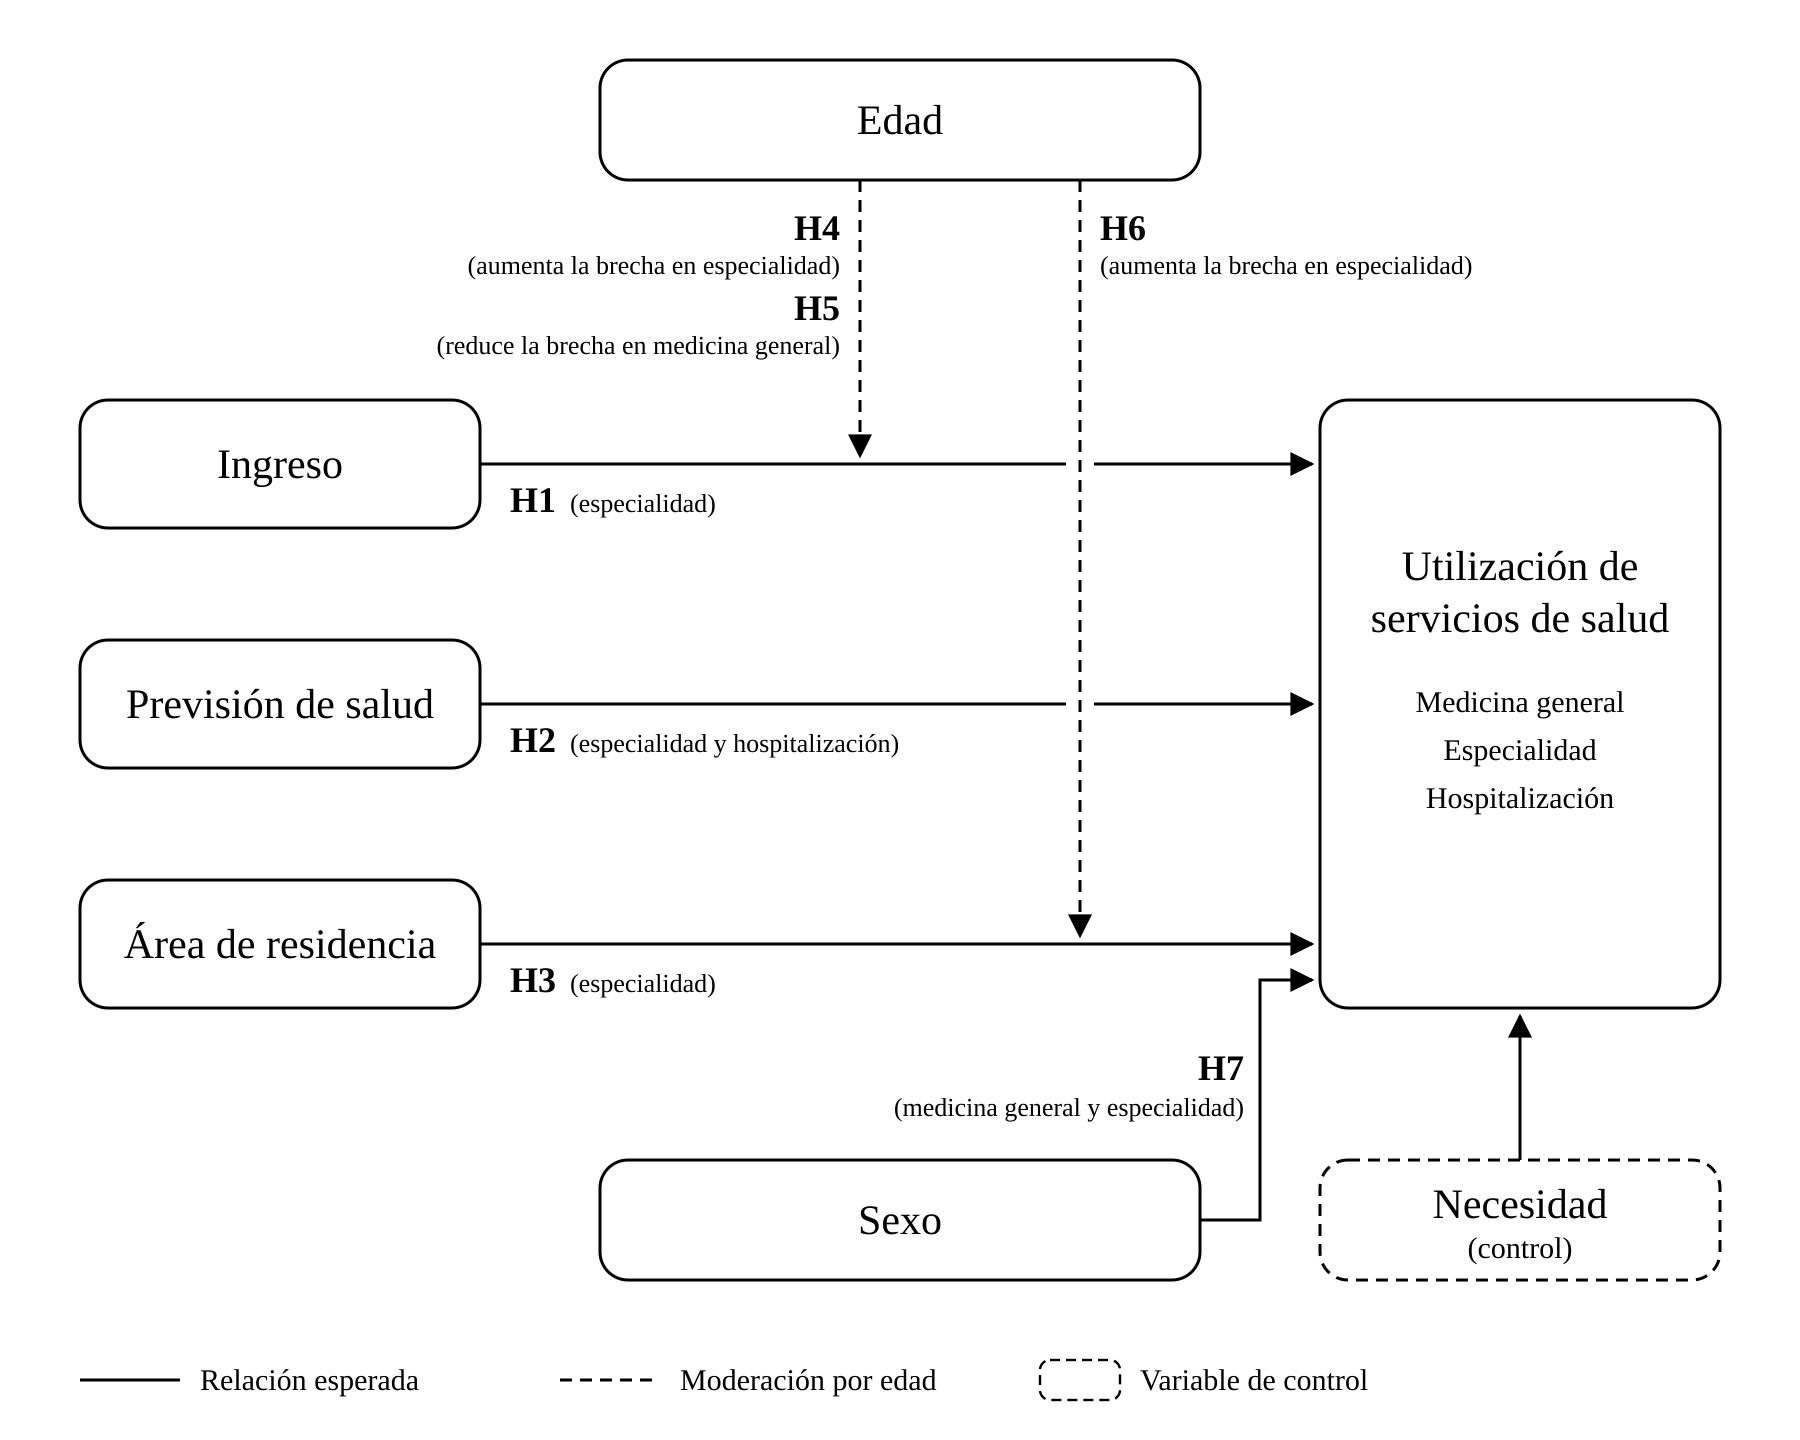
\includegraphics[width=0.95\linewidth,height=\textheight,keepaspectratio]{assets/diagrama_hipotesis_final_v2.png}

}

\end{figure}%

\emph{Nota.} Las hipótesis H2, H3 y H7 plantean una mayor utilización
entre las personas afiliadas a Isapre, residentes en zonas urbanas y
mujeres, respectivamente. Las hipótesis exploratorias (He1 a He7) se
presentan en el texto.

\bookmarksetup{startatroot}

\chapter{Metodología}\label{metodologuxeda}

\section{Datos}\label{datos}

La investigación tendrá un enfoque cuantitativo, observacional y
transversal. Se utilizará como fuente principal de datos la
\href{https://observatorio.ministeriodesarrollosocial.gob.cl/encuesta-casen-2024}{Encuesta
de Caracterización Socioeconómica Nacional (CASEN) 2024}, desarrollada
por el Ministerio de Desarrollo Social y Familia. La encuesta recopila
información sobre aspectos demográficos, módulos de salud, educación,
vivienda, trabajo e ingresos, que permite conocer periódicamente la
situación de los hogares y de la población, especialmente de aquella en
situación de pobreza y de aquellos grupos definidos como prioritarios
por la política social, además de evaluar el impacto de la política
social (\citeproc{ref-mdsf_informe_2026}{Ministerio de Desarrollo Social
y Familia, 2026}). La base de microdatos y su documentación metodológica
son de acceso público a través del Observatorio Social del MDSF.

La población objetivo de la encuesta corresponde a las personas que
residen en viviendas particulares ocupadas del territorio nacional.
Quedan excluidas las personas que residen en viviendas colectivas, como
establecimientos de larga estadía para personas mayores u hospitales, y
las áreas clasificadas como especiales por el INE en el Marco Muestral
de Viviendas (MMV) 2021, entre ellas diez comunas completas
(\citeproc{ref-mdsf_informe_2026}{Ministerio de Desarrollo Social y
Familia, 2026, p. 29}).

El diseño muestral es probabilístico, estratificado y bietápico. Los
estratos se definieron por la combinación de comuna, área y nivel
socioeconómico de las Unidades Primarias de Muestreo (UPM); en cada
estrato, la selección de UPM se realizó de forma independiente, y la
unidad final de selección es la vivienda
(\citeproc{ref-mdsf_informe_2026}{Ministerio de Desarrollo Social y
Familia, 2026}). La recolección de datos se realizó entre el 1 de
noviembre de 2024 y el 2 de febrero de 2025, mediante entrevistas
presenciales asistidas por dispositivos electrónicos a una persona
informante integrante del hogar de 18 años o más, que cuenta con la
información necesaria para completar la encuesta, quien responde la
totalidad de los módulos del cuestionario en representación de todos los
integrantes del hogar, conforme a los criterios establecidos en el
manual de campo (\citeproc{ref-mdsf_informe_2026}{Ministerio de
Desarrollo Social y Familia, 2026, pp. 14, 56}). La muestra lograda
alcanzó 218.367 personas, pertenecientes a 78.654 hogares, con una tasa
de respuesta de 74,1\% (\citeproc{ref-mdsf_informe_2026}{Ministerio de
Desarrollo Social y Familia, 2026}).

Para esta investigación, la unidad de análisis son las personas. El
estudio se realiza en dos etapas: primero se describen la población y la
utilización según grupo de edad, ingreso, previsión y territorio
mediante porcentajes ponderados, y luego se estiman modelos
multivariados. Ambas etapas se restringen a la población de 18 años y
más (\emph{N} = 172.309), porque la utilización de los menores de 18
años depende principalmente de las decisiones y los recursos de las
personas adultas del hogar.

Todas las estimaciones estadísticas se realizarán aplicando los factores
de expansión poblacional (expr) y las variables de estratos (varstrat) y
conglomerados (varunit), considerando el diseño muestral complejo de la
CASEN, para garantizar que los resultados sean representativos a nivel
nacional. Las restricciones de la muestra se realizarán mediante
estimación de subpoblaciones, y no eliminando casos, para estimar
correctamente la varianza. Las respuestas ``no sabe'' y ``no responde''
se tratarán como datos perdidos. Para que los modelos anidados sean
comparables, todos se estimarán sobre la misma muestra analítica: las
personas con información completa en todas las variables del modelo más
completo.

\section{Variables}\label{variables}

\subsection{Variables dependientes}\label{variables-dependientes}

Para esta investigación, las variables dependientes corresponden a tres
indicadores de utilización declarada de servicios de salud, construidos
como variables dicotómicas (1 = utilizó el servicio en el período de
referencia; 0 = no lo utilizó).

Estos indicadores miden utilización efectivamente declarada, y no
permiten evaluar la oportunidad, la pertinencia ni la calidad de la
atención. Dado que los períodos de referencia difieren entre servicios,
la comparación entre ellos se realiza sobre patrones y no sobre niveles
de utilización.

\begin{longtable}[t]{>{\raggedright\arraybackslash}p{4cm}>{\raggedright\arraybackslash}p{2.5cm}>{\raggedright\arraybackslash}p{2.5cm}>{\raggedright\arraybackslash}p{6cm}}

\caption{\label{tbl-dependientes}Variables dependientes}

\tabularnewline

\toprule
Variable & Código CASEN & Período de referencia & Observaciones\\
\midrule
\endfirsthead
\multicolumn{4}{@{}l}{\textit{(continued)}}\\
\toprule
Variable & Código CASEN & Período de referencia & Observaciones\\
\midrule
\endhead

\endfoot
\bottomrule
\endlastfoot
\textbf{Atención de medicina general} & \ttfamily{s20a\_preg} & Últimos 3 meses & -\\
\textbf{Atención de especialidad} & \ttfamily{s23a\_preg} & Últimos 3 meses & -\\
\textbf{Hospitalización o intervención quirúrgica} & \ttfamily{s27a} & Últimos 12 meses & Se tratan como datos perdidos (NA) las hospitalizaciones por embarazo, parto o cesárea (0,8 \%).\\*

\end{longtable}

\subsection{Variables independientes}\label{variables-independientes}

Las variables independientes se organizarán de acuerdo con las
dimensiones del Modelo Conductual de Utilización de los Servicios de
Salud de Andersen (\citeproc{ref-andersen_revisiting_1995}{1995},
\citeproc{ref-andersen_national_2008}{2008}), distinguiendo entre
factores predisponentes, facilitadores y de necesidad.

\begin{longtable}[t]{>{\raggedright\arraybackslash}p{3cm}>{\raggedright\arraybackslash}p{3.5cm}>{\raggedright\arraybackslash}p{2cm}>{\raggedright\arraybackslash}p{6.5cm}}

\caption{\label{tbl-operacionalizacion}Variables independientes}

\tabularnewline

\toprule
Dimensión (Andersen) & Variable & Código CASEN & Categorías / Operacionalización\\
\midrule
\endfirsthead
\multicolumn{4}{@{}l}{\textit{(continued)}}\\
\toprule
Dimensión (Andersen) & Variable & Código CASEN & Categorías / Operacionalización\\
\midrule
\endhead

\endfoot
\bottomrule
\endlastfoot
 & Edad & \ttfamily{edad} & 5 tramos: 18-34, 35-49, 50-64, 65-79 y 80+ años. Referencia: 18-34.\\
\nopagebreak
 & Sexo & \ttfamily{sexo} & Nominal dicotómica: 1 = hombre, 2 = mujer. Referencia: hombre.\\
\nopagebreak
\multirow[t]{-2}{3cm}[\normalbaselineskip]{\raggedright\arraybackslash \textbf{Factores Predisponentes}} & Nivel educacional & \ttfamily{educc} & Ordinal (4 categorías): básica incompleta o menos (0-1), básica completa o media incompleta (2-3), media completa (4) y educación superior (5-6). Valores negativos (-88) son perdidos.\\
\cmidrule{1-4}\pagebreak[0]
 & Problema de salud, enfermedad o accidente & \ttfamily{s16} & Dicotómica (Sí/No): declara algún problema de salud, enfermedad o accidente en los últimos 3 meses.\\
\nopagebreak
\multirow[t]{-1}{3cm}[\normalbaselineskip]{\raggedright\arraybackslash \textbf{Factores de Necesidad}} & Limitación funcional & \ttfamily{h7a a h7f} & Dicotómica (Sí/No): "Sí" indica mucha dificultad o imposibilidad en al menos uno de los 6 dominios (criterio Washington Group).\\
\cmidrule{1-4}\pagebreak[0]
 & Sistema previsional de salud & \ttfamily{s13} & Dicotómica: Fonasa e Isapre. Referencia: Fonasa. Se excluyen FF.AA. y del Orden, ninguno y otro.\\
\nopagebreak
\multirow[t]{-1}{3cm}[\normalbaselineskip]{\raggedright\arraybackslash \textbf{Facilitadores Individuales}} & Ingreso total per cápita del hogar & \ttfamily{ypchtotcor} & Quintiles (Q1 a Q5) calculados con el factor de expansión sobre la población total. Referencia: Q1.\\
\cmidrule{1-4}\pagebreak[0]
 & Región de residencia & \ttfamily{region} & Nominal categórica: regiones del país. Referencia: Región Metropolitana.\\
\nopagebreak
 & Área geográfica & \ttfamily{area} & Nominal dicotómica: 1 = urbano, 2 = rural. Referencia: urbano.\\
\nopagebreak
\multirow[t]{-2}{3cm}[\normalbaselineskip]{\raggedright\arraybackslash \textbf{Facilitadores Territoriales}} & Proximidad a centro de salud & \ttfamily{v35c} & Dicotómica: 1 = sí (< 20 cuadras o 2,5 km), 2 = no.\\*

\end{longtable}

La edad se agrupa en cinco tramos para captar relaciones no lineales con
la utilización. Aunque la Ley N° 19.828 define como adulta mayor a la
persona de 60 años y más, se utiliza el umbral de 65 años para mantener
la comparabilidad con las cifras del INE citadas en la introducción, y
el de 80 años corresponde a la cuarta edad que define la misma ley.
Siguiendo a Siguiendo a Andersen
(\citeproc{ref-andersen_revisiting_1995}{1995}), la educación se trata
como una característica de la estructura social y no como un recurso
material.

Los dos indicadores de necesidad corresponden a necesidad percibida, y
no evaluada por criterios profesionales
(\citeproc{ref-andersen_national_2008}{Andersen, 2008}). Ambos son
declarados por el informante del hogar y no equivalen a una evaluación
clínica. El período de referencia del problema de salud reciente
coincide con el de la atención de medicina general y de especialidad.

Las personas con otro sistema previsional quedan fuera del análisis, por
lo que los resultados de los modelos se refieren a la población adulta
afiliada a Fonasa o Isapre. Los tramos de Fonasa no se desagregan porque
se definen por ingreso, que ya se incluye en el modelo. Se utiliza el
ingreso per cápita porque permite comparar hogares de distinto tamaño y
porque el gasto en salud se resuelve en gran medida en el hogar. Se
emplea el ingreso total, que incluye las transferencias monetarias del
Estado, por su relevancia para la población mayor, y se agrupa en
quintiles porque estos describen la posición relativa, permiten capturar
relaciones no lineales y reducen el efecto de los valores extremos. Como
prueba de robustez, los modelos se estimarán también con el ingreso
autónomo per cápita del hogar, lo que permitirá evaluar en qué medida
las transferencias modifican la relación entre el ingreso y la
utilización, especialmente en la población mayor.

Finalmente, la proximidad declarada a un centro de salud constituye una
aproximación a la cercanía territorial de los servicios y no una medida
directa del acceso efectivo.

\subsection{Valores perdidos}\label{valores-perdidos}

Los porcentajes de valores perdidos se calcularon sobre los 172.309
adultos de la muestra, sin ponderar. Son de 0,0 \% en el área de
residencia; 0,1 \% en el quintil de ingreso y en la limitación
funcional; 0,2 \% en la cercanía a un centro de salud, en la atención de
medicina general y en la de especialidad; 0,3 \% en el nivel
educacional; y 0,7 \% en el problema de salud reciente. La edad, el sexo
y la región no presentan valores perdidos.

La previsión y la hospitalización tienen porcentajes mayores. En la
previsión, el 4,4 \% de los adultos queda fuera del análisis: el 4,0 \%
tiene otra previsión, que se excluye por decisión metodológica, y el 0,4
\% no tiene dato. En la hospitalización, el 1,0 \% queda fuera: el 0,8
\% corresponde a hospitalizaciones por embarazo, parto o cesárea, que se
excluyen por corresponder a una lógica distinta a la de necesidad
asociada a la edad, y el 0,2 \% no tiene dato.

\section{Estrategia de análisis}\label{estrategia-de-anuxe1lisis}

Se utilizarán modelos de regresión logística binaria para estimar la
probabilidad de utilización de cada uno de los tres tipos de servicios
de salud (medicina general, atención de especialidad y hospitalización o
intervención quirúrgica) en la población de 18 años y más. Todas las
estimaciones incorporan los factores de expansión y el diseño muestral
de CASEN 2024. Para cada persona \(i\) y servicio \(j\), se modela

\[
\text{logit}(p_{ij}) = \ln\left(\frac{p_{ij}}{1-p_{ij}}\right)
\]

donde \(p_{ij}\) es la probabilidad de que la persona \(i\) haya
utilizado el servicio \(j\). Se estimará un conjunto de modelos anidados
y secuenciales para cada resultado.

\textbf{Modelo 1: factores predisponentes.} Incorpora edad, sexo y nivel
educacional.

\begin{equation}\protect\phantomsection\label{eq-m1}{
\text{logit}(p_{ij}) = \beta_0 + \mathbf{P}_i'\boldsymbol{\beta}_P
}\end{equation}

\textbf{Modelo 2: factores de necesidad.} Agrega el problema de salud
reciente y la limitación funcional.

\begin{equation}\protect\phantomsection\label{eq-m2}{
\text{logit}(p_{ij}) = \beta_0 + \mathbf{P}_i'\boldsymbol{\beta}_P + \mathbf{N}_i'\boldsymbol{\beta}_N
}\end{equation}

\textbf{Modelo 3: factores facilitadores.} Agrega el ingreso y la
previsión de salud (H1 y H2; objetivo 2) y el área de residencia y la
proximidad a un centro de salud (H3; objetivo 3). La región de
residencia se incluye como variable de control. Con este modelo se
evalúan además He1 y He2 (objetivos 2 y 3) y la diferencia por sexo (H7;
objetivo 1).

\begin{equation}\protect\phantomsection\label{eq-m3}{
\text{logit}(p_{ij}) = \beta_0 + \mathbf{P}_i'\boldsymbol{\beta}_P + \mathbf{N}_i'\boldsymbol{\beta}_N + \mathbf{F}_i'\boldsymbol{\beta}_F + \mathbf{T}_i'\boldsymbol{\beta}_T
}\end{equation}

\textbf{Modelo 4: interacciones con la edad.} Para cada servicio, agrega
por separado la interacción entre el grupo de edad y el ingreso (H4, H5
y He3), la previsión de salud (He4) y el área de residencia (H6)
(objetivo 4).

\emph{4a. Edad × ingreso (H4, H5 y He3)}

\begin{equation}\protect\phantomsection\label{eq-m4a}{
\text{logit}(p_{ij}) = \text{M3} + \sum_{g=2}^{5}\sum_{q=2}^{5}\gamma_{gq}\,(E_{gi}\times Q_{qi})
}\end{equation}

\emph{4b. Edad × previsión (He4)}

\begin{equation}\protect\phantomsection\label{eq-m4b}{
\text{logit}(p_{ij}) = \text{M3} + \sum_{g=2}^{5}\gamma_{g}\,(E_{gi}\times \text{Isapre}_i)
}\end{equation}

\emph{4c. Edad × área de residencia (H6)}

\begin{equation}\protect\phantomsection\label{eq-m4c}{
\text{logit}(p_{ij}) = \text{M3} + \sum_{g=2}^{5}\gamma_{g}\,(E_{gi}\times \text{Rural}_i)
}\end{equation}

\textbf{Modelo 5: interacciones con el sexo.} Agrega por separado la
interacción entre el sexo y el ingreso (He5), la previsión de salud
(He6) y el área de residencia (He7) (objetivo 5).

\emph{5a. Sexo × ingreso (He5)}

\begin{equation}\protect\phantomsection\label{eq-m5a}{
\text{logit}(p_{ij}) = \text{M3} + \sum_{q=2}^{5}\delta_{q}\,(\text{Mujer}_i\times Q_{qi})
}\end{equation}

\emph{5b. Sexo × previsión (He6)}

\begin{equation}\protect\phantomsection\label{eq-m5b}{
\text{logit}(p_{ij}) = \text{M3} + \delta\,(\text{Mujer}_i\times \text{Isapre}_i)
}\end{equation}

\emph{5c. Sexo × área de residencia (He7)}

\begin{equation}\protect\phantomsection\label{eq-m5c}{
\text{logit}(p_{ij}) = \text{M3} + \delta\,(\text{Mujer}_i\times \text{Rural}_i)
}\end{equation}

Donde \(\mathbf{P}_i\) corresponde al vector de factores predisponentes
(grupo de edad, sexo y nivel educacional), \(\mathbf{N}_i\) al de
factores de necesidad (problema de salud reciente y limitación
funcional), \(\mathbf{F}_i\) al de facilitadores individuales (quintil
de ingreso y previsión de salud) y \(\mathbf{T}_i\) al de facilitadores
territoriales (área de residencia, cercanía a un centro de salud y
región). M3 representa todos los términos del Modelo 3. \(E_{gi}\)
indica el grupo de edad \(g\) y \(Q_{qi}\) el quintil de ingreso \(q\).
Las categorías de referencia son el grupo de 18 a 34 años, los hombres,
el primer quintil, la afiliación a Fonasa y la zona urbana. Los
coeficientes \(\gamma\) y \(\delta\) indican en qué medida la asociación
de cada factor con la utilización difiere entre grupos de edad o entre
hombres y mujeres.

Cada modelo de interacción conserva todos los términos del Modelo 3, y
la significancia de cada interacción se evaluará mediante pruebas
conjuntas que consideran el diseño muestral. Las interacciones se
interpretarán mediante probabilidades predichas por grupo de edad,
comparando si las diferencias entre las categorías de cada factor
aumentan o disminuyen a medida que aumenta la edad
(\citeproc{ref-mize_best_2019}{Mize, 2019}).

Previo a la estimación, se evaluará la multicolinealidad entre nivel
educacional, ingreso y previsión de salud mediante el factor de
inflación de la varianza (VIF).

\bookmarksetup{startatroot}

\chapter{Resultados descriptivos}\label{resultados-descriptivos}

\textbf{Tabla 1. Caracterización de la población de 18 años y más (\%)}

La Tabla 1 presenta las características de la población de 18 años y más
según los factores predisponentes, facilitadores y de necesidad. En
términos de la estructura etaria, el 31,7\% de la población adulta tiene
entre 18 y 34 años y el 27,8\% entre 35 y 49 años, mientras que las
personas de 65 años y más representan el 17,9\%, de las cuales el 4,1\%
tiene 80 años o más. En la distribución por sexo, los hombres
representan un 48,9\% y las mujeres un 51,1\%. El nivel educacional se
distribuye principalmente en educación superior con un 41,7\%, seguida
de un 31\% con educación media completa frente a valores inferiores de
educación básica completa o media incompleta con 17,4\% y básica
incompleta o menos con un 9,9\%.

Respecto de la necesidad, el 19,1\% declara haber tenido un problema de
salud en los últimos tres meses y el 11,5\% presenta limitación
funcional. En cuanto a los factores facilitadores, Fonasa concentra la
mayoría de los casos con un 82,6\% frente a un 13,3\% afiliado a Isapres
y un 4,1\% con otra previsión, grupo que se excluye de los modelos
multivariados . En cuanto al territorio, el 88,5\% reside en zonas
urbanas y el 81,8\% declara contar con un centro de salud cercano a su
vivienda. Por último, la distribución por quintiles de ingreso varía
desde un 16,3\% en el quintil de menores ingresos (Q1) hasta un 22\% en
los quintiles Q4 y Q5. Esto se debe a que los quintiles se calcularon
sobre la población total y a que los menores de 18 años se concentran en
los quintiles de menores ingresos, en parte porque el ingreso per cápita
es menor en los hogares con más integrantes.

\textbackslash begin\{table\}{[}!h{]} \centering
\textbackslash caption\{\label{tab:unnamed-chunk-2}Tabla 1.
Caracterización de la población de 18 años y más (\%)\} \centering
\resizebox{\ifdim\width>\linewidth\linewidth\else\width\fi}{!}{
\fontsize{10}{12}\selectfont
\begin{tabular}[t]{lll}
\toprule
\textbf{Variable} & \textbf{Categoría} & \textbf{\%}\\
\midrule
Grupo de edad & 18-34 & 31,7\\
 & 35-49 & 27,8\\
 & 50-64 & 22,6\\
 & 65-79 & 13,8\\
 & 80+ & 4,1\\
Sexo & Hombre & 48,9\\
 & Mujer & 51,1\\
Nivel educacional & Básica incompleta o menos & 9,9\\
 & Básica completa o media incompleta & 17,4\\
 & Media completa & 31,0\\
 & Superior & 41,7\\
Problema de salud reciente & Sí & 19,1\\
 & No & 80,9\\
Limitación funcional & Sí & 11,5\\
 & No & 88,5\\
Previsión de salud & FONASA & 82,6\\
 & Isapre & 13,3\\
 & Otra previsión & 4,1\\
Quintil de ingreso & Q1 & 16,3\\
 & Q2 & 18,8\\
 & Q3 & 20,9\\
 & Q4 & 22,0\\
 & Q5 & 22,0\\
Área de residencia & Urbano & 88,5\\
 & Rural & 11,5\\
Centro de salud a menos de 20 cuadras o 2,5 km & Sí & 81,8\\
 & No & 18,2\\
\bottomrule
\end{tabular}} \textbackslash end\{table\}

\emph{Nota.} Elaboración propia con datos de CASEN 2024.

\textbf{Tabla 2. Necesidad de salud y utilización de servicios según
grupo de edad (\%)}

La Tabla 2 muestra la distribución de los dos indicadores de necesidad y
los tres tipos de utilización de los servicios de salud según los grupos
etarios. Ambos indicadores de necesidad aumentan progresivamente con la
edad, en especial la limitación funcional, que pasa de 3,8\% en el grupo
de 18 a 34 años a 54,2\% en las personas de 80 años y más. La
utilización también aumenta con la edad, aunque en menor magnitud. Entre
esos mismos grupos, la medicina general aumenta 25,7 puntos porcentuales
(de 19,0\% a 44,7\%), la especialidad 15,8 puntos (de 16,1\% a 31,9\%) y
la hospitalización 10,0 puntos (de 4,7\% a 14,7\%), mientras que la
limitación funcional aumenta 50,4 puntos. Esta diferencia es más marcada
en las edades más altas. Entre los grupos de 65 a 79 años y de 80 años y
más, la limitación funcional aumenta 28,1 puntos, mientras que la
medicina general lo hace en 4,4 puntos y la especialidad en 2,9 puntos.

\textbackslash begin\{table\}{[}!h{]} \centering
\textbackslash caption\{\label{tab:unnamed-chunk-3}Tabla 2. Necesidad de
salud y utilización de servicios según grupo de edad (\%)\} \centering
\resizebox{\ifdim\width>\linewidth\linewidth\else\width\fi}{!}{
\fontsize{10}{12}\selectfont
\begin{tabular}[t]{llllll}
\toprule
\textbf{Grupo de edad} & \textbf{Problema reciente} & \textbf{Limitación funcional} & \textbf{Medicina general} & \textbf{Especialidad} & \textbf{Hospitalización}\\
\midrule
18-34 & 13,7 & 3,8 & 19,0 & 16,1 & 4,7\\
35-49 & 17,4 & 5,1 & 24,4 & 19,6 & 6,9\\
50-64 & 21,5 & 13,4 & 31,3 & 22,2 & 8,7\\
65-79 & 26,9 & 26,1 & 40,3 & 29,0 & 12,2\\
80+ & 31,7 & 54,2 & 44,7 & 31,9 & 14,7\\
Total 18 años y más & 19,1 & 11,5 & 27,3 & 20,9 & 7,7\\
\bottomrule
\end{tabular}} \textbackslash end\{table\}

\emph{Nota.} Elaboración propia con datos de CASEN 2024.

\textbf{Tabla 3. Utilización de servicios según ingreso, previsión y
territorio (\%)}

La Tabla 3 muestra el porcentaje de personas que utilizan cada servicio
según su quintil de ingreso, su previsión de salud y su territorio de
residencia. En los tres servicios la utilización aumenta con el quintil
de ingreso, y el gradiente más marcado se observa en la atención de
especialidad, que va de 14,3\% en el Q1 a 30,4\% en el Q5; en medicina
general va de 22,0\% a 31,2\% y en hospitalización de 6,5\% a 8,9\%. Las
personas afiliadas a Isapre utilizan más los tres servicios que las
afiliadas a Fonasa, con la mayor diferencia en la atención de
especialidad (33,7\% frente a 19,1\%). En cuanto al territorio, residir
en zona rural se asocia con menor utilización en los tres servicios,
especialmente en especialidad (15,8\% frente a 21,5\% en zona urbana).
La cercanía a un centro de salud muestra diferencias menores: quienes no
cuentan con uno cercano utilizan menos la medicina general (26,0\%
frente a 27,6\%) y la especialidad (18,5\% frente a 21,4\%), sin
diferencias en hospitalización (7,7\% en ambos casos). Dado que estas
cifras corresponden a porcentajes no ajustados (es decir, que no
consideran las necesidades de salud ni la relación entre los propios
factores) el efecto neto de cada variable será evaluado posteriormente
mediante los modelos multivariados.

\textbackslash begin\{table\}{[}!h{]} \centering
\textbackslash caption\{\label{tab:unnamed-chunk-4}Tabla 3. Utilización
de servicios según ingreso, previsión y territorio (\%)\} \centering
\resizebox{\ifdim\width>\linewidth\linewidth\else\width\fi}{!}{
\fontsize{10}{12}\selectfont
\begin{tabular}[t]{lllll}
\toprule
\textbf{Variable} & \textbf{Categoría} & \textbf{Medicina general} & \textbf{Especialidad} & \textbf{Hospitalización}\\
\midrule
Quintil de ingreso & Q1 & 22,0 & 14,3 & 6,5\\
 & Q2 & 25,4 & 16,8 & 7,1\\
 & Q3 & 27,4 & 18,6 & 7,7\\
 & Q4 & 28,9 & 21,9 & 7,8\\
 & Q5 & 31,2 & 30,4 & 8,9\\
Previsión de salud & FONASA & 27,1 & 19,1 & 7,4\\
 & Isapre & 30,6 & 33,7 & 9,7\\
Área de residencia & Urbano & 27,6 & 21,5 & 7,8\\
 & Rural & 25,0 & 15,8 & 6,8\\
Centro de salud cercano & Sí & 27,6 & 21,4 & 7,7\\
 & No & 26,0 & 18,5 & 7,7\\
\bottomrule
\end{tabular}} \textbackslash end\{table\}

\emph{Nota.} Elaboración propia con datos de CASEN 2024.

\bookmarksetup{startatroot}

\chapter{Referencias
bibliográficas}\label{referencias-bibliogruxe1ficas}

\protect\phantomsection\label{refs}
\begin{CSLReferences}{1}{0}
\bibitem[\citeproctext]{ref-aday_framework_1974}
Aday, L. A., \& Andersen, R. (1974). A framework for the study of access
to medical care. \emph{Health Services Research}, \emph{9}(3), 208-220.
\url{https://pmc.ncbi.nlm.nih.gov/articles/instance/1071804/pdf/hsresearch00560-0030.pdf}

\bibitem[\citeproctext]{ref-albala_envejecimiento_2020}
Albala, C. (2020). El envejecimiento de la población chilena y los
desafíos para la salud y el bienestar de las personas mayores.
\emph{Revista Médica Clínica Las Condes}, \emph{31}(1), 7-12.
\url{https://doi.org/10.1016/j.rmclc.2019.12.001}

\bibitem[\citeproctext]{ref-andersen_revisiting_1995}
Andersen, R. M. (1995). Revisiting the behavioral model and access to
medical care: {Does} it matter? \emph{Journal of Health and Social
Behavior}, \emph{36}(1), 1-10. \url{https://doi.org/10.2307/2137284}

\bibitem[\citeproctext]{ref-andersen_national_2008}
Andersen, R. M. (2008). National health surveys and the behavioral model
of health services use. \emph{Medical Care}, \emph{46}(7), 647-653.
\url{https://doi.org/10.1097/MLR.0b013e31817a835d}

\bibitem[\citeproctext]{ref-asadi-lari_need_2003}
Asadi-Lari, M., Packham, C., \& Gray, D. (2003). Need for redefining
needs. \emph{Health and Quality of Life Outcomes}, \emph{1}.
\url{https://doi.org/10.1186/1477-7525-1-34}

\bibitem[\citeproctext]{ref-atal_etal_2026}
Atal, J. P., Larroucau, T., Muñoz, P., \& Otero, C. (2026).
\emph{Physicians' occupational licensing and the quantity-quality
trade-off}. Documento de trabajo.

\bibitem[\citeproctext]{ref-bancomundial_medicos_sf}
Banco Mundial. (s.~f.). \emph{Médicos (cada 1.000 personas) - {Chile}}.
Recuperado 18 de octubre de 2026, de
\url{https://datos.bancomundial.org/indicador/SH.MED.PHYS.ZS?locations=CL}

\bibitem[\citeproctext]{ref-bassdelcampo_universalizacion_2025}
Bass del Campo, C. (2025). Universalización de Atención Primaria en
Chile: una política lamentablemente regresiva. \emph{Cuadernos Médico
Sociales}, \emph{65}(1), 53-65.
\url{https://doi.org/10.56116/cms.v65.n1.2025.2209}

\bibitem[\citeproctext]{ref-bcn_ley_sf}
Biblioteca del Congreso Nacional de Chile. (s.~f.). \emph{Ley de
urgencia en salud. Ley Fácil}. Recuperado 27 de octubre de 2026, de
\url{https://www.bcn.cl/portal/leyfacil/recurso/ley-de-urgencia-en-salud}

\bibitem[\citeproctext]{ref-blanco_enfoque_2011}
Blanco, M. (2011). El enfoque del curso de vida: orígenes y desarrollo.
\emph{Revista Latinoamericana de Población}, \emph{5}(8), 5-31.
\url{https://doi.org/10.31406/relap2011.v5.i1.n8.1}

\bibitem[\citeproctext]{ref-chackiel_envejecimiento_2000}
Chackiel, J. (2000). \emph{El envejecimiento de la población
latinoamericana: ¿hacia una relación de dependencia favorable?} Comisión
Económica para América Latina y el Caribe.
\url{https://repositorio.cepal.org/server/api/core/bitstreams/c15fd12a-15b2-4b61-91f6-4863270ae3d8/content}

\bibitem[\citeproctext]{ref-chovarvera_desigualdad_2014}
Chovar Vera, A., Vásquez Lavín, F., \& Paraje, G. (2014). Desigualdad e
inequidad en la utilización de servicios médicos según grupos etarios en
Chile, 2000--2011. \emph{Revista Panamericana de Salud Pública},
\emph{36}(3), 171-178.
\url{https://www.scielosp.org/pdf/rpsp/2014.v36n3/171-178/es}

\bibitem[\citeproctext]{ref-clinicasdechile_dimensionamiento_2025}
Clínicas de Chile. (2025). \emph{Dimensionamiento de la oferta de salud
en Chile 2024}. Asociación de Clínicas de Chile AG.
\url{https://www.clinicasdechile.cl/wp-content/uploads/2025/12/Dimensionamiento-del-Sector-Salud-en-Chile-\%E2\%80\%93-Cifras-a-2024.pdf}

\bibitem[\citeproctext]{ref-cepal_acerca_sf}
Comisión Económica para América Latina y el Caribe. (s.~f.).
\emph{Acerca de envejecimiento}. Recuperado
\url{https://www.cepal.org/es/temas/envejecimiento/acerca-envejecimiento}

\bibitem[\citeproctext]{ref-cepal_impactos_2026}
Comisión Económica para América Latina y el Caribe. (2026).
\emph{Impactos del cambio demográfico en América Latina y el Caribe:
Retos y opciones para la política pública} (LC/CRPD.6/3).

\bibitem[\citeproctext]{ref-dannefer_cumulative_2003}
Dannefer, D. (2003). Cumulative advantage/disadvantage and the life
course: {Cross-fertilizing} age and social science theory. \emph{The
Journals of Gerontology Series B: Psychological Sciences and Social
Sciences}, \emph{58}(6), S327-S337.
\url{https://doi.org/10.1093/geronb/58.6.S327}

\bibitem[\citeproctext]{ref-deis_defunciones_2026}
Departamento de Estadísticas e Información de Salud. (2026).
\emph{Defunciones y mortalidad por capítulo {CIE-10} de causa básica de
defunción y año. Tablero de datos} {[}Dataset{]}. Ministerio de Salud de
Chile.
\url{https://informesdeis.minsal.cl/SASVisualAnalytics/?reportUri=\%2Freports\%2Freports\%2F4013de47-a3c2-47b8-8547-075525e4f819&sectionIndex=0&sso_guest=true&reportViewOnly=true&reportContextBar=false&sas-welcome=false}

\bibitem[\citeproctext]{ref-ferraro_aging_2009}
Ferraro, K. F., \& Shippee, T. P. (2009). Aging and cumulative
inequality: {How} does inequality get under the skin? \emph{The
Gerontologist}, \emph{49}(3), 333-343.
\url{https://doi.org/10.1093/geront/gnp034}

\bibitem[\citeproctext]{ref-fuenzalida_analisis_2023}
Fuenzalida, M., Crespo, F., \& Lanio, I. (2023). Análisis de la
cobertura geográfica de camas hospitalarias públicas en Chile.
\emph{Revista Geográfica de Chile Terra Australis}, \emph{59}, 92-101.
\url{https://doi.org/10.23854/07199562.2023591.fuenzalida}

\bibitem[\citeproctext]{ref-gattini_sistema_2018}
Gattini, C. (2018). \emph{El sistema de salud en Chile}. Observatorio
Chileno de Salud Pública, Universidad de Chile.
\url{https://www.ochisap.cl/wp-content/uploads/2022/04/Sistema_Salud_Chile_Gattini_2018.pdf}

\bibitem[\citeproctext]{ref-goldstein_sistema_2018}
Goldstein, E. (2018). \emph{El sistema de salud en Chile y la Atención
Primaria de Salud municipal: Marco para un debate sobre
desmunicipalización}. Biblioteca del Congreso Nacional de Chile.
\url{https://obtienearchivo.bcn.cl/obtienearchivo?id=repositorio/10221/26811/2/BCN_Gobernanza_salud_y_demunicip_para_reposit_final.pdf}

\bibitem[\citeproctext]{ref-goldstein_resena_2024}
Goldstein, E. (2024). \emph{Reseña sobre la Ley Corta de ISAPRES de 2024
(Ley N° 21.674)}. Biblioteca del Congreso Nacional de Chile.
\url{https://obtienearchivo.bcn.cl/obtienearchivo?id=repositorio/10221/36273/1/BCN__Resena_Ley_Corta_Isapres_2024__final.pdf}

\bibitem[\citeproctext]{ref-gonzalez_estructura_2019}
González, C., Castillo-Laborde, C., \& Matute, I. (Eds.). (2019).
\emph{Estructura y funcionamiento del sistema de salud chileno}.
Universidad del Desarrollo. \url{http://hdl.handle.net/11447/2895}

\bibitem[\citeproctext]{ref-henriquez_desigualdades_2015}
Henríquez, J., \& Velasco, C. (2015). \emph{Las desigualdades en la
atención médica en los últimos 20 años} (Propuestas de Política Pública
No. 13). Centro de Estudios Públicos.

\bibitem[\citeproctext]{ref-huaiquilaf-jorquera_medicos_2026}
Huaiquilaf-Jorquera, S., Riedemann Gonzalez, J. P., Castillo Mora, J.
A., \& Arancibia Luna, M. J. (2026). Médicos especialistas en Chile:
Análisis de la situación 2024. \emph{Revista Médica de Chile},
\emph{154}(3).
\url{https://www.revistamedicadechile.cl/index.php/rmedica/article/view/11531}

\bibitem[\citeproctext]{ref-huenchuan_proteccion_2011}
Huenchuan, S. (2011). \emph{La protección de la salud en el marco de la
dinámica demográfica y los derechos} {[}Serie Población y Desarrollo{]}.
Comisión Económica para América Latina y el Caribe.

\bibitem[\citeproctext]{ref-huenchuan_envejecimiento_2016}
Huenchuan, S. (Ed.). (2016). \emph{Envejecimiento e institucionalidad
pública en América Latina y el Caribe: conceptos, metodologías y casos
prácticos}. Comisión Económica para América Latina y el Caribe.
\url{https://www.cepal.org/es/publicaciones/40197-envejecimiento-institucionalidad-publica-america-latina-caribe-conceptos}

\bibitem[\citeproctext]{ref-huenchuan_envejecimiento_2018}
Huenchuan, S. (Ed.). (2018). \emph{Envejecimiento, personas mayores y
Agenda 2030 para el Desarrollo Sostenible: perspectiva regional y de
derechos humanos}. Comisión Económica para América Latina y el Caribe.
\url{https://repositorio.cepal.org/bitstream/handle/11362/44369/1/S1800629_es.pdf}

\bibitem[\citeproctext]{ref-hugorojas_envejecimiento_2022}
Hugo Rojas, F., Rodríguez Canache, L., \& Rodríguez León, J. (2022).
\emph{Envejecimiento en Chile: Evolución, características de las
personas mayores y desafíos demográficos para la población}
{[}Documentos de Trabajo{]}. Instituto Nacional de Estadísticas.
\url{https://www.ine.gob.cl/docs/default-source/documentos-de-trabajo/envejecimiento-en-chile-evolucion-y-caracteristicas-de-las-personas-mayores.pdf?sfvrsn=fa394551_2}

\bibitem[\citeproctext]{ref-ine_transicion_2022}
Instituto Nacional de Estadísticas. (2022). \emph{Transición demográfica
y el envejecimiento de la población en Chile: Evolución, características
de las personas mayores y desafíos demográficos para la población.
Presentación}. Conferencia ciudadana, Subdepartamento de Demografía.
\url{https://www.ine.gob.cl/docs/default-source/conferencias/evolucion-demografica/conferencias-ciudadanas-evolucion-demografica-en-chile.pdf}

\bibitem[\citeproctext]{ref-ine_cifras_2025}
Instituto Nacional de Estadísticas. (2025a). \emph{Cifras provisionales
de estadísticas vitales confirman disminución de nacimientos en 2024.
Noticia}.
\url{https://www.ine.gob.cl/sala-de-prensa/prensa/general/noticia/2025/05/15/cifras-provisionales-de-estad\%C3\%ADsticas-vitales-confirman-disminuci\%C3\%B3n-de-nacimientos-en-2024}

\bibitem[\citeproctext]{ref-ine_primeros_2025}
Instituto Nacional de Estadísticas. (2025b). \emph{Primeros resultados
del Censo 2024: 18.480.432 personas fueron censadas en Chile,
manteniéndose la tendencia de envejecimiento de la población}.
\url{https://censo2024.ine.gob.cl/primeros-resultados-del-censo-2024-18-480-432-personas-fueron-censadas-en-chile-manteniendose-la-tendencia-de-envejecimiento-de-la-poblacion/}

\bibitem[\citeproctext]{ref-ine_estimaciones_2026}
Instituto Nacional de Estadísticas. (2026). \emph{Estimaciones y
proyecciones de población 1992-2070: Base 2024. Presentación de
resultados}. Instituto Nacional de Estadísticas.
\url{https://www.ine.gob.cl/docs/default-source/proyecciones-de-poblacion/publicaciones-y-anuarios/proyecci\%C3\%B3n-base-2024/estimaciones-y-proyecciones-de-poblaci\%C3\%B3n-1992-2070_base-2024_presentaci\%C3\%B3n-de-resultados.pdf}

\bibitem[\citeproctext]{ref-lantz_socioeconomic_2001}
Lantz, P. M. (2001). Socioeconomic status and health care. En N. J.
Smelser \& P. B. Baltes (Eds.), \emph{International encyclopedia of the
social \& behavioral sciences} (pp. 14558-14562). Elsevier.
\url{https://doi.org/10.1016/B0-08-043076-7/03828-6}

\bibitem[\citeproctext]{ref-levesque_patient-centred_2013}
Levesque, J.-F., Harris, M. F., \& Russell, G. (2013). Patient-centred
access to health care: {Conceptualising} access at the interface of
health systems and populations. \emph{International Journal for Equity
in Health}, \emph{12}. \url{https://doi.org/10.1186/1475-9276-12-18}

\bibitem[\citeproctext]{ref-_ley_2002}
Ley N° 19.828. (2002, septiembre 27). \emph{Crea el Servicio Nacional
del Adulto Mayor}. Ministerio Secretaría General de la Presidencia.
\url{https://www.bcn.cl/leychile/navegar?idNorma=202950}

\bibitem[\citeproctext]{ref-menares_munoz_2025}
Menares, F., \& Muñoz, P. (2025). The impact of standardized
disease-specific healthcare coverage. \emph{Journal of Public
Economics}, \emph{242}, 105312.
\url{https://doi.org/10.1016/j.jpubeco.2025.105312}

\bibitem[\citeproctext]{ref-mendoza-sassi_utilizacion_2001}
Mendoza-Sassi, R., \& Béria, J. U. (2001). Utilización de los servicios
de salud: una revisión sistemática sobre los factores relacionados.
\emph{Cadernos de Saúde Pública}, \emph{17}(4), 819-832.
\url{https://www.scielosp.org/article/csp/2001.v17n4/819-832/}

\bibitem[\citeproctext]{ref-mdsf_informe_2026}
Ministerio de Desarrollo Social y Familia. (2026). \emph{Informe
metodológico Casen 2024}. Observatorio Social.
\url{https://observatorio.ministeriodesarrollosocial.gob.cl/storage/docs/casen/2024/Informe_metodologico_casen_2024.pdf}

\bibitem[\citeproctext]{ref-minsal_informe_2023}
Ministerio de Salud, Departamento de Epidemiología. (2023).
\emph{Informe vigilancia enfermedades no transmisibles 2023}. Ministerio
de Salud.
\url{https://epi.minsal.cl/wp-content/uploads/2025/05/INFORME_NACIONAL_VENT_CHILE.pdf}

\bibitem[\citeproctext]{ref-minsal_encuesta_2025}
Ministerio de Salud, Departamento de Epidemiología. (2025).
\emph{Encuesta Nacional de Calidad de Vida y Salud ({ENCAVI}) 2023-2024:
Resultados. Presentación de diapositivas}.
\url{https://epi.minsal.cl/wp-content/uploads/2026/07/PPT_ENCAVI_2023_24.pdf}

\bibitem[\citeproctext]{ref-minsal_levantamiento_2025}
Ministerio de Salud, \& Organización Panamericana de la Salud. (2025).
\emph{Levantamiento de información de Postas de Salud Rural}. Ministerio
de Salud.
\url{https://www.paho.org/sites/default/files/2026/09/minsal-ops-2025-levantamiento-informacion-psr-final-comprimido.pdf}

\bibitem[\citeproctext]{ref-mize_best_2019}
Mize, T. D. (2019). Best practices for estimating, interpreting, and
presenting nonlinear interaction effects. \emph{Sociological Science},
\emph{6}, 81-117. \url{https://doi.org/10.15195/v6.a4}

\bibitem[\citeproctext]{ref-moscosocuaresma_determinantes_2017}
Moscoso Cuaresma, J. R., Cárdenas, E., \& Juárez, C. (2017).
\emph{Determinantes sociales en salud}. Universidad Peruana de Ciencias
Aplicadas.
\url{https://www.researchgate.net/profile/Julio-Ricardo-Moscoso-Cuaresma/publication/385822723_Determinantes_sociales_en_salud/links/6736a966a78ba469f0617e2a/Determinantes-sociales-en-salud.pdf}

\bibitem[\citeproctext]{ref-munoz_otero_2025}
Muñoz, P., \& Otero, C. (2025). Managers and public hospital
performance. \emph{American Economic Review}, \emph{115}(11), 4040-4074.
\url{https://doi.org/10.1257/aer.20240615}

\bibitem[\citeproctext]{ref-nunez_equity_2013}
Núñez, A., \& Chi, C. (2013). Equity in health care utilization in
{Chile}. \emph{International Journal for Equity in Health}, \emph{12}.
\url{https://doi.org/10.1186/1475-9276-12-58}

\bibitem[\citeproctext]{ref-observatorio_envejecer_2023}
Observatorio del Envejecimiento UC-Confuturo. (2023). \emph{Envejecer en
la ruralidad: Explorando una realidad invisibilizada} (Año 5, vol. No.
29). Observatorio del Envejecimiento UC-Confuturo.

\bibitem[\citeproctext]{ref-observatorio_viviendo_2025}
Observatorio del Envejecimiento UC-Confuturo. (2025). \emph{Viviendo con
enfermedades crónicas: Perspectivas desde la población mayor} (Año 6,
vol. No. 36). Observatorio del Envejecimiento UC-Confuturo.

\bibitem[\citeproctext]{ref-olguin_niveles_2025}
Olguín, C. (2025, octubre 20). \emph{Niveles de atención en salud: El
rol de la atención secundaria y terciaria}. ADIPA.
\url{https://adipa.cl/noticias/niveles-de-atencion-en-salud-el-rol-de-la-atencion-secundaria-y-terciaria/}

\bibitem[\citeproctext]{ref-oecd_health_2025}
Organisation for Economic Co-operation and Development. (2025).
\emph{Health at a Glance 2025: {Country} notes --- {Chile}}.
\url{https://www.oecd.org/es/publications/2025/11/health-at-a-glance-2025-country-notes_2f94481e/chile_b440e042.html}

\bibitem[\citeproctext]{ref-paraje_health_2012}
Paraje, G., \& Vásquez, F. (2012). Health equity in an unequal country:
{The} use of medical services in {Chile}. \emph{International Journal
for Equity in Health}, \emph{11}.
\url{https://doi.org/10.1186/1475-9276-11-81}

\bibitem[\citeproctext]{ref-penchansky_concept_1981}
Penchansky, R., \& Thomas, J. W. (1981). The concept of access:
{Definition} and relationship to consumer satisfaction. \emph{Medical
Care}, \emph{19}(2), 127-140.
\url{https://doi.org/10.1097/00005650-198102000-00001}

\bibitem[\citeproctext]{ref-pnud_desigualdad_2018}
Programa de las Naciones Unidas para el Desarrollo. (2018).
\emph{Desigualdad regional en Chile: Ingresos, salud y educación en
perspectiva territorial}. Programa de las Naciones Unidas para el
Desarrollo.

\bibitem[\citeproctext]{ref-nodo_comunidades_2021}
Proyecto NODO. (2021). \emph{Comunidades y entornos rurales en Chile.
Análisis y perspectivas sobre población mayor}. Sistema de las Naciones
Unidas en Chile.

\bibitem[\citeproctext]{ref-robledomarin_teorias_2021}
Robledo Marín, C. A., \& Orejuela Gómez, J. J. (2021). Teorías de la
sociología del envejecimiento y la vejez. \emph{Revista Guillermo de
Ockham}, \emph{18}(1), 95-102.
\url{https://doi.org/10.21500/22563202.4660}

\bibitem[\citeproctext]{ref-rodriguezsantana_need_2023}
Rodriguez Santana, I., Mason, A., Gutacker, N., Kasteridis, P., Santos,
R., \& Rice, N. (2023). Need, demand, supply in health care: {Working}
definitions, and their implications for defining access. \emph{Health
Economics, Policy and Law}, \emph{18}(1), 1-13.
\url{https://doi.org/10.1017/S1744133121000293}

\bibitem[\citeproctext]{ref-ssms_rol_sf}
Servicio de Salud Metropolitano Sur. (s.~f.). \emph{Rol de la red
asistencial}. Ministerio de Salud, Gobierno de Chile. Recuperado 18 de
octubre de 2026, de \url{https://ssms.gob.cl/rol-de-la-red-asistencial/}

\bibitem[\citeproctext]{ref-superintendencia_como_sf}
Superintendencia de Salud. (s.~f.-a). \emph{Cómo funciona el Sistema de
Salud en Chile}. Ministerio de Salud, Gobierno de Chile. Recuperado 20
de octubre de 2026, de
\url{https://www.superdesalud.gob.cl/orientacion-en-salud/como-funciona-el-sistema-de-salud-en-chile/}

\bibitem[\citeproctext]{ref-superintendencia_garantias_sf}
Superintendencia de Salud. (s.~f.-b). \emph{Garantías Explícitas en
Salud ({GES})}. Gobierno de Chile. Recuperado 20 de octubre de 2026, de
\url{https://www.superdesalud.gob.cl/tax-temas-de-orientacion/garantias-explicitas-en-salud-ges-1962/}

\bibitem[\citeproctext]{ref-superintendencia_caracterizacion_2023}
Superintendencia de Salud. (2023). \emph{Caracterización de las
especialidades médicas en Chile en 2022}. Ministerio de Salud.
\url{https://www.superdesalud.gob.cl/documentacion/666/articles-26547_recurso_1.pdf}

\bibitem[\citeproctext]{ref-travassos_revisao_2004}
Travassos, C., \& Martins, M. (2004). Uma revisão sobre os conceitos de
acesso e utilização de serviços de saúde. \emph{Cadernos de Saúde
Pública}, \emph{20}(Supl. 2), S190-S198.
\url{https://www.scielo.br/j/csp/a/PkyrsjDrZWwzzPVJJPbbXtQ/}

\bibitem[\citeproctext]{ref-turra_transicion_2021}
Turra, C. M., \& Fernandes, F. (2021). \emph{La transición demográfica:
Oportunidades y desafíos en la senda hacia el logro de los Objetivos de
Desarrollo Sostenible en América Latina y el Caribe} (LC/TS.2020/105).
Comisión Económica para América Latina y el Caribe.
\url{https://www.cepal.org/es/publicaciones/46805-la-transicion-demografica-oportunidades-desafios-la-senda-logro-objetivos}

\bibitem[\citeproctext]{ref-unitednations_world_2020}
United Nations, Department of Economic and Social Affairs, Population
Division. (2020). \emph{World population ageing 2019}
(ST/ESA/SER.A/444). United Nations.
\url{https://digitallibrary.un.org/record/3907988/files/WorldPopulationAgeing2019-Report.pdf}

\bibitem[\citeproctext]{ref-vasquez_income-related_2013}
Vásquez, F., Paraje, G., \& Estay, M. (2013). Income-related inequality
in health and health care utilization in {Chile}, 2000--2009.
\emph{Revista Panamericana de Salud Pública}, \emph{33}(2), 98-106.
\url{https://doi.org/10.1590/S1020-49892013000200004}

\bibitem[\citeproctext]{ref-vignolo_niveles_2011}
Vignolo, J., Vacarezza, M., Álvarez, C., \& Sosa, A. (2011). Niveles de
atención, de prevención y atención primaria de la salud. \emph{Archivos
de Medicina Interna}, \emph{33}(1), 7-11.
\url{http://www.scielo.edu.uy/scielo.php?script=sci_arttext&pid=S1688-423X2011000100003&lng=es&tlng=es}

\end{CSLReferences}


\backmatter

% --- Cuerpo del libro (capítulos) en arábigos ---
\mainmatter
\pagestyle{scrheadings}

% --- (Opcional) Estilo del índice general ---
% \addtocontents{toc}{\protect\thispagestyle{plain}}


\end{document}
